\documentclass[11pt]{article}
\usepackage{amsmath, amssymb, amsthm}
\usepackage{geometry}
\usepackage{float}
\usepackage{setspace}
\usepackage{booktabs}
\usepackage{graphicx}
\usepackage{natbib}
\usepackage{siunitx}
\usepackage{empheq}
\usepackage{pdfpages}
\usepackage{longtable}
\usepackage{threeparttable}
\usepackage{adjustbox}
\usepackage{xcolor}
\usepackage{comment}
\usepackage[colorlinks=true, linkcolor=blue, citecolor=blue, urlcolor=blue]{hyperref}
\excludecomment{notes} % or \includecomment{notes}

% Theorem-style environments
\theoremstyle{plain}
\newtheorem{lemma}{Lemma}
\newtheorem{proposition}{Proposition}

% Optional: remarks (roman text)
\theoremstyle{remark}
\newtheorem{remark}{Remark}

% Optional: section-based numbering (recommended)
\numberwithin{lemma}{section}
\numberwithin{proposition}{section}
\newtheorem{corollary}{Corollary}
\numberwithin{corollary}{section}

% ---------- Revision markup: new/changed text appears in blue ----------
\definecolor{RevBlue}{RGB}{0,0,205}
\newcommand{\rev}[1]{{\color{RevBlue}#1}}
\newenvironment{revblock}{\par\begingroup\color{RevBlue}}{\endgroup\par}

\bibliographystyle{apalike}

\geometry{margin=1in}

\setstretch{1.2}
\title{Trade Tariffs and Exchange Rates:\\
Revisiting Conventional Wisdom in a Three-Country Framework}

\author{
Jason Lu\thanks{International Monetary Fund, Research Department. Email: {\tt jlu2@imf.org}} 
\and 
Dimitre Milkov\thanks{International Monetary Fund, Research Department. Email: {\tt dmilkov@imf.org}}
}

\date{First draft: November 10, 2025 \\ This version: \today \footnote{An interactive companion dashboard is available at {\tt https://jasonzhixinglu.github.io/tariff-exchange-rates/}.}}

\begin{document}

\maketitle

\begin{abstract}
\rev{The exchange rate in the class of models underlying the conventional tariff--appreciation prediction is the common-currency relative wage, and therefore the bilateral terms of trade --- the object the preferential-trade-agreement literature has studied since Viner. A selective tariff is formally a preference in favor of the untariffed partner, so that literature bears directly on the tariff--exchange-rate question; we illustrate the connection with minimal theory in the smallest multilateral setting. Doing so yields two results. First, the connection is invisible under the standard Armington specification: with a common elasticity across all tradable varieties, the conventional appreciation result survives the three-country extension \emph{as a theorem}, for every elasticity, at any realistic home bias. Second, it fails once the home--import elasticity $\eta$ and the cross-origin elasticity $\rho$ are separated, and we derive the exact threshold at which it fails: the home currency depreciates against untariffed partners if and only if $\rho > \rho^* = 3\left[1+\alpha_D(\eta-1)-\alpha_T(1-\alpha_D)\right]$. At US-realistic parameters and 2025-scale tariffs the threshold is approximately $3$, inside the range of measured cross-origin elasticities; in a near-symmetric trade war the ambiguity resolves and both belligerents depreciate against the bystander. A calibration to the 2025 US--China episode, disciplined by the tariffs in force at each date, matches the April 2025 pattern --- modest dollar appreciation against the renminbi alongside depreciation against the euro --- at central elasticities, while showing that the near-uniform tariffs of late 2025 cannot account for the year-end dollar weakness through the trade channel. Consequently, bilateral appreciation against a tariffed partner is not evidence of broad currency strength, and observed multilateral depreciation during a tariff episode cannot be attributed to financial or convenience-yield channels on the strength of the two-country prior alone.}
\end{abstract}

\noindent\textbf{Keywords:} Trade Tariffs, Exchange Rates, Trade Diversion, Open-Economy Equilibrium

\newpage
\section{Introduction}

What happens to exchange rates when a country imposes trade tariffs? In practice, exchange rate responses are context dependent and reflect a confluence of factors, but the conventional wisdom derived from a two-country trade model predicts an unambiguous currency appreciation for the tariff-imposing country. The intuition is that tariffs lead to a substitution of expenditure toward domestic goods, and hence an improvement in the bilateral trade balance and an appreciation of the home currency. This result has a long lineage, beginning with \cite{lerner1936symmetry}, who established the equivalence between import tariffs and export taxes in a two-country setting and the closely related link between tariffs and exchange rate adjustment under flexible rates. \cite{metzler1949tariffs} extended the analysis to a two-country general equilibrium framework emphasizing the terms-of-trade channel, and \cite{mundell1961flexible} embedded these ideas in an open-economy macroeconomic framework showing that tariff-induced currency appreciation offsets the trade-balance effects of commercial policy under flexible exchange rates. Modern micro-founded treatments reinforce the same conclusion: \cite{obstfeld1996foundations} and \cite{corsetti2001welfare} provided the analytical toolkit for studying policy transmission through terms-of-trade and exchange rate adjustments in fully intertemporal settings with optimizing agents, demonstrating that the relative price channels identified in the classical literature remain operative across a wide range of frameworks.

The way this mechanism works is as follows. A tariff imposed by country $A$ on imports from country $B$ raises the consumer price of $B$'s tradable goods in country $A$. Holding the exchange rate fixed, the immediate effect is an expenditure-switching response: households in country $A$ substitute away from imported goods toward domestically produced goods. This contraction in import demand improves country $A$'s trade balance at the prevailing exchange rate, requiring an appreciation of country $A$'s currency in equilibrium to restore trade balance. Depending on the treatment of tariff revenue, income effects may reinforce this mechanism by further reducing import demand as real income falls. More generally, any force that lowers import expenditures at a given exchange rate shifts the trade balance condition in the same direction. While additional channels, for example through adjustments in export prices or firm markups, may also be relevant depending on the context, they are not essential for the result.

Empirical evidence from recent tariff episodes has complicated this picture. \cite{jeanne2024extent} studies the 2018--19 US-China trade tariffs using a calibrated small open economy model and shows that the model generates only a small appreciation of the USD alongside a large depreciation of the RMB, broadly matching the observed exchange rate pattern during the episode. They also conduct a high-frequency event study showing that US tariff announcements led to an immediate USD appreciation, while Chinese retaliation announcements had no significant exchange rate effects. \cite{khalil2024us} argues that tariff-induced increases in trade policy uncertainty contributed to the appreciation of the USD during the same episode, operating through higher safe-haven demand for US Treasuries — an additional channel that reinforces the conventional prediction. The 2025 episode is harder to reconcile with the conventional wisdom. \cite{cardani2025exchange} studies the April 2025 US reciprocal tariffs using a three-country DSGE open economy model and documents that the dollar weakened after the announcement, contrary to the conventional prediction. They attribute this to a decline in the convenience yield of US Treasuries, driven by weaker growth expectations and heightened policy uncertainty, which triggered portfolio outflows from the US. Taken together, the 2018--19 episode is broadly consistent with the conventional wisdom, possibly amplified by financial safe-haven flows, while the 2025 episode is not, and the existing literature has turned primarily to financial and convenience-yield channels to account for the gap. \rev{Related recent work reinforces this reading: \cite{kalemli2025} rationalize the 2025 dollar depreciation through tariff \emph{uncertainty} operating on risk premia, and \cite{werning2025} study tariffs as cost-push shocks for optimal monetary policy. On the trade side, \cite{darracq2026} quantify the third-country spillovers of the 2025 escalation in a three-country New Keynesian model, and \cite{liqiu2022} estimate the two-elasticity Armington structure we use below and show that conflating the two elasticities badly distorts third-country welfare calculations --- but neither provides the analytical sign characterization for exchange rates that is our focus. Yet the event-study evidence of \cite{corsetti2025} points to a systematically \emph{trade-shaped} pattern: the dollar appreciates when US tariffs are unilateral and depreciates when trading partners retaliate --- precisely the configuration dependence that, as we show below, real trade channels alone generate in a multilateral setting.}

\begin{revblock}
The starting point of this paper is an observation about what the exchange rate \emph{is} in the class of models that generates the conventional prediction. With one factor, linear technology, and balanced trade, the nominal exchange rate is, up to a constant, the common-currency \emph{relative wage} --- and, because producer prices are unit labor costs, simultaneously the bilateral \emph{terms of trade}. Three names for one number. And an isolated tariff by $A$ on $B$, holding $A$'s tariff on $C$ at zero, is formally a \emph{preferential arrangement} in favor of $C$: up to the level of the external tariff and the treatment of revenue, ``raise $\tau_{AB}$'' and ``cut $\tau_{AC}$'' are the same discriminatory wedge. It follows that a literature that has tracked the third-country terms-of-trade consequences of discriminatory tariffs since \cite{viner1950} --- through \cite{mundell1964} on tariff preferences, \cite{kempwan1976}, the terms-of-trade externality framework of \cite{bagwell1999, bagwell2002}, and the excluded-country price effects measured by \cite{changwinters2002} --- bears directly on the tariff--exchange-rate question, as does the quantitative literature that computes relative wages under arbitrary tariff vectors \citep{caliendo2015, ossa2014, costinot2014}. The contribution of this paper is to make that connection explicit and to illustrate it with minimal theory in the smallest multilateral setting; the inferential step for the 2025 debate --- that these literatures imply ``the dollar should depreciate against the euro'' is a possible consequence of a purely real tariff shock --- is one neither literature has had occasion to take. Section~\ref{sec:relwage} develops the equivalence. The analysis is purely real: no nominal rigidities, no financial frictions, no uncertainty channels.

When country $A$ imposes a tariff on imports from country $B$, the first-order expenditure-switching response need not be directed solely toward domestic goods: expenditure can be diverted toward imports from the untariffed third country $C$, deteriorating the bilateral balance between $A$ and $C$ and generating depreciation pressure on $A$'s currency. Whether this diversion force can \emph{dominate} turns out to hinge on a distinction that a single trade elasticity cannot express. Our first result is an impossibility theorem: in a three-country CES model in which one elasticity $\sigma$ governs substitution across all tradable varieties, the conventional appreciation result survives for \emph{every} value of $\sigma$ whenever the home share of tradable expenditure is realistic. The reason is that a higher $\sigma$ strengthens diversion toward $C$ and conventional home-versus-import expenditure switching in the same proportion: the threshold the diversion force must clear rises exactly as fast as the force itself. The flat-CES intuition, we argue, is precisely why the profession has remained anchored on the two-country prior.

The reversal requires separating the two margins. In a nested demand system with a macro (home-versus-import) elasticity $\eta$ and a micro (cross-origin) elasticity $\rho$, we derive a closed-form threshold, $\rho^* = 3\left[1 + \alpha_D(\eta - 1) - \alpha_T(1-\alpha_D)\right]$, such that an isolated tariff depreciates $A$'s currency against the untariffed third country if and only if $\rho > \rho^*$. The threshold is increasing in home bias $\alpha_D$ and in the macro elasticity $\eta$, decreasing in the tradable expenditure share $\alpha_T$ and in the size of the third country, and \emph{decreasing} in the size of the tariff itself, so the local threshold is a conservative bound at 2025-scale tariffs. At US-realistic parameters the threshold is approximately $4$ for marginal tariffs and approximately $3$ at 2025-scale tariffs, inside the range of measured cross-origin elasticities \citep{feenstra2018, broda2006, liqiu2022, fajgelbaum2024trade}: the reversal is not a knife-edge curiosity, but it is invisible to any calibration that conflates the two elasticities. Finally, in a bilateral trade war the two forces reinforce from the bystander's perspective, and both belligerents' currencies depreciate against the untariffed third country --- unambiguously for near-symmetric wars, with magnitude increasing in $\rho$.
\end{revblock}

The model abstracts from several features present in a more realistic model of multilateral trade, and the results should be interpreted accordingly. First, the three-country framework represents a minimal multilateral environment. Real trade networks involve many countries simultaneously, and the interactions among bilateral exchange rates in a fully multilateral model can be considerably more complex than what we characterize here. Second, the model abstracts from richer production structures, including capital, endogenous labor supply, human capital, intermediate goods, and cross-country technological differences, all of which shape the transmission of tariff shocks in quantitative trade models. Third, the model is static and real: there are no nominal rigidities in consumer prices, no role for invoicing currency, and no intertemporal dynamics. A large literature examines how invoicing currency and nominal price rigidities shape the transmission of tariff shocks to exchange rates and trade flows, which our model does not speak to.\footnote{\cite{devereux2003monetary} shows that the currency of price-setting determines exchange rate passthrough, with complete passthrough under producer currency pricing and attenuated passthrough under local currency pricing. \cite{gopinath2020dominant} extends this framework by introducing a third invoicing currency, and \cite{bergin2023macroeconomic} show that the resulting asymmetries can create monetary policy tradeoffs that potentially reverse standard predictions about the exchange rate response to tariff shocks.} Our exchange rate predictions should therefore be interpreted as long-run equilibrium outcomes in which prices have fully adjusted and current account imbalances cannot persist indefinitely.

Introducing short-run dynamics would require nominal frictions, sticky prices, and a financial account that allows trade imbalances to be offset by capital flows. In practice, financial flows are large relative to trade flows and often dominate exchange rate movements at business cycle frequencies, which is one reason observed exchange rate changes may differ substantially from the model's long-run predictions. Given these limitations, the purpose of this paper is not to deliver a realistic framework for quantitative analysis but to establish a conceptual point: one cannot appeal to the conventional two-country wisdom to conclude that any observed depreciation must reflect financial or non-trade factors. In a multilateral setting, real trade channels alone are sufficient to generate depreciation of the tariff-imposing country's currency against untariffed trading partners, and the qualitative direction of the multilateral exchange rate response depends on the structure of trade as much as on financial conditions.

\rev{The rest of the paper is organized as follows. Section~\ref{sec:twocountry} develops the two-country model, establishes the conventional appreciation result, shows that its robustness is exactly the robustness of the Marshall--Lerner condition, makes explicit the equivalence between the exchange rate, the relative wage, and the terms of trade in this model class, and states the scope of the exercise and the purpose of each modelling restriction. Section~\ref{sec:threecountry} introduces the three-country model, analyzes the three tariff configurations, and presents the two main results: the impossibility theorem for the single-elasticity model and the reversal threshold $\rho^*$ for the nested model. Section~\ref{sec:calibration} presents a quantitative illustration calibrated to the 2025 US tariff episode. Section~\ref{sec:conclusion} concludes.}

\section{The Two-Country Model}
\label{sec:twocountry}

We consider a static two-country, two-sector, one-factor model in which a single nominal exchange rate equilibrates international trade. We first derive the conventional result that tariffs lead to an appreciation of the tariff-imposing country's currency, obtain a closed-form expression for the equilibrium exchange rate, and then establish the robustness of this result using a general monotonicity argument that does not rely on specific functional form assumptions.

\subsection{The Two-Country Conventional Wisdom}
\label{sec:twocountry_cw}

Countries are indexed by $i \in \{A,B\}$ and goods by $g \in \{T_A, T_B, N\}$, where $T_i$ denotes the tradable good produced in country $i$ and $N$ denotes a non-tradable good that is produced and consumed domestically. Labor is the only factor of production and is immobile across countries.

\subsubsection{Firms}

Each good is produced using a linear technology. Output in the tradable and non-tradable sectors satisfies
\begin{equation}
Y_{T_i} = A_{T_i} L_{T_i}, \qquad Y_{N_i} = A_{N_i} L_{N_i}, \qquad L_{T_i} + L_{N_i} = L_i,
\end{equation}
where $A_{T_i}$ and $A_{N_i}$ denote sectoral labor productivities and $L_i$ is the total labor endowment in country $i$. Markets are perfectly competitive. With linear production technologies, firms earn zero profits in equilibrium, and wages in each country are equalized across sectors. We normalize the producer prices of tradable goods to one, so that $P_{T_A}=P_{T_B}=1$, and maintain this normalization throughout the analysis. Under this normalization, equilibrium wages satisfy
\begin{equation}
w_i = A_{T_i} = P_{N_i} A_{N_i},
\label{eq:wage}
\end{equation}
which implies $P_{N_i} = A_{T_i}/A_{N_i}$, so that nontradable prices are pinned down by the ratio of sectoral productivities.

\subsubsection{Households}

Households in each country consume the domestically produced tradable good, the tradable good produced abroad, and a non-tradable good produced locally. Let $C_{T_i i}$ denote country $i$'s consumption of its own tradable good, $C_{T_j i}$ its consumption of the tradable good produced in the other country $j \neq i$, and $C_{N_i}$ its consumption of the local non-tradable good. Let $e$ denote the nominal exchange rate, defined as units of country $A$'s currency per unit of country $B$'s currency, so that the domestic-currency price of $T_B$ in country $A$ is $eP_{T_B}$ and the domestic-currency price of $T_A$ in country $B$ is $P_{T_A}/e$. Under free trade, household income equals wage income, $I_i = w_i L_i$. The household budget constraints are
\begin{equation}
w_A L_A = P_{T_A}\, C_{T_A A} + e P_{T_B}\, C_{T_B A} + P_{N_A}\, C_{N_A},
\label{eq:budget_A}
\end{equation}
\begin{equation}
w_B L_B = \frac{P_{T_A}}{e}\, C_{T_A B} + P_{T_B}\, C_{T_B B} + P_{N_B}\, C_{N_B}.
\label{eq:budget_B}
\end{equation}
Preferences in each country are Cobb--Douglas over the two tradable goods and the local non-tradable good, with expenditure shares $\alpha_{T_A}$, $\alpha_{T_B}$, and $\alpha_N = 1 - \alpha_{T_A} - \alpha_{T_B}$ on goods $T_A$, $T_B$, and $N$ respectively, where $\alpha_{T_j}$ denotes the common weight on good $T_j$ in both countries' utility functions. Utility in country $i$ is given by
\[
U_i = C_{T_A i}^{\alpha_{T_A}}\, C_{T_B i}^{\alpha_{T_B}}\, C_{N_i}^{\,\alpha_N}.
\]
Utility maximization subject to the budget constraints implies that households allocate constant expenditure shares across goods. Equilibrium expenditures satisfy
\begin{equation}
P_{T_A}\, C_{T_A i} = \alpha_{T_A}\, I_i, \qquad P_{T_B}^{(i)}\, C_{T_B i} = \alpha_{T_B}\, I_i, \qquad P_{N_i}\, C_{N_i} = \alpha_N\, I_i,
\label{eq:expenditures}
\end{equation}
where $P_{T_B}^{(i)}$ denotes the domestic-currency price of $T_B$ faced by country $i$, equal to $eP_{T_B}$ in country $A$ and $P_{T_B}$ in country $B$ under free trade. These expenditure-share conditions hold generally, with $I_i = w_i L_i$ under free trade; once tariffs are introduced in Section~\ref{sec:tariffs}, $I_i$ includes rebated tariff revenue and $I_i \neq w_i L_i$ in general. The corresponding consumption quantities are
\begin{equation}
C_{T_A i} = \frac{\alpha_{T_A}\, I_i}{P_{T_A}}, \qquad C_{T_B i} = \frac{\alpha_{T_B}\, I_i}{P_{T_B}^{(i)}}, \qquad C_{N_i} = \frac{\alpha_N\, I_i}{P_{N_i}}.
\label{eq:demands}
\end{equation}

\subsubsection{Market Clearing and Equilibrium}

In equilibrium, markets clear in each country for non-tradable and tradable goods, and international trade is balanced. Non-tradable goods are produced and consumed domestically; for each country $i \in \{A,B\}$, market clearing requires $Y_{N_i} = C_{N_i}$. Using the production technology, the wage condition $P_{N_i} = w_i/A_{N_i}$, and Cobb--Douglas demand, equilibrium labor allocations satisfy
\begin{equation}
\frac{L_{N_i}}{L_i} = \alpha_N, \qquad \frac{L_{T_i}}{L_i} = 1 - \alpha_N = \alpha_{T_A} + \alpha_{T_B}.
\end{equation}
Each tradable variety is produced in only one country and consumed in both. For tradable good $T_i$, global market clearing requires $Y_{T_i} = C_{T_i i} + C_{T_i j}$, which using \eqref{eq:demands} gives
\begin{equation}
A_{T_A} L_{T_A} = \frac{\alpha_{T_A}\, I_A}{P_{T_A}} + \frac{\alpha_{T_A}\, I_B}{P_{T_A}/e}, \qquad
A_{T_B} L_{T_B} = \frac{\alpha_{T_B}\, I_B}{P_{T_B}} + \frac{\alpha_{T_B}\, I_A}{e\, P_{T_B}},
\label{eq:T_world_clearing}
\end{equation}
where $P_{T_A}/e$ is the price of $T_A$ in country $B$'s currency and $eP_{T_B}$ is the price of $T_B$ in country $A$'s currency. Trade balances are measured in each country's own currency; for country $A$, export revenues are $P_{T_A} C_{T_A B}$ and import expenditures are $eP_{T_B} C_{T_B A}$, giving
\begin{equation}
\mathrm{TB}_A = P_{T_A}\, C_{T_A B} - e P_{T_B}\, C_{T_B A}.
\label{eq:TB}
\end{equation}
Imposing balanced trade $\mathrm{TB}_A = 0$ and substituting \eqref{eq:demands} yields the equilibrium condition
\begin{equation}
\alpha_{T_A}\, w_B L_B = \alpha_{T_B}\, e\, w_A L_A.
\label{eq:TB_condition}
\end{equation}
By Walras' Law, satisfying \eqref{eq:TB_condition} for country $A$ ensures global market clearing, so the equilibrium exchange rate is fully determined by a single trade balance condition.

\subsubsection{Imposing Tariffs in the Two-Country Model}
\label{sec:tariffs}

We introduce an ad valorem tariff $\tau \ge 0$ levied by country $A$ on imports of the tradable good $T_B$. The tariff raises the consumer price of $T_B$ in country $A$ to $(1+\tau)e P_{T_B}$, while producers in country $B$ continue to receive the world price $P_{T_B} = 1$, so the tariff wedge $\tau e P_{T_B}$ is collected as revenue by country $A$'s government and rebated lump-sum to households. The household budget constraint in country $A$ becomes
\begin{equation}
I_A = P_{T_A}\, C_{T_A A} + (1+\tau)e P_{T_B}\, C_{T_B A} + P_{N_A}\, C_{N_A},
\end{equation}
where $I_A \equiv w_A L_A + T_A^{\mathrm{rev}}$ is total household income and tariff revenue is $T_A^{\mathrm{rev}} = \tau e P_{T_B}\, C_{T_B A}$. Substituting $T_A^{\mathrm{rev}}$ into the definition of $I_A$ and using the Cobb--Douglas expenditure share condition $C_{T_B A} = \alpha_{T_B} I_A / [(1+\tau)e P_{T_B}]$, income solves to the closed form
\begin{equation}
I_A = \frac{w_A L_A}{1 - \dfrac{\alpha_{T_B}\,\tau}{1+\tau}},
\label{eq:income_tariff}
\end{equation}
which exceeds wage income $w_A L_A$ for any $\tau > 0$, reflecting the rebated tariff revenue. Equilibrium consumption demands in country $A$ are then
\begin{align}
C_{T_A A} &= \frac{\alpha_{T_A}\, I_A}{P_{T_A}}, \\
C_{T_B A} &= \frac{\alpha_{T_B}\, I_A}{(1+\tau)\,e\,P_{T_B}}, \\
C_{N_A}   &= \frac{\alpha_N\, I_A}{P_{N_A}}.
\end{align}
In country $B$, which does not impose tariffs, income equals wage income and consumption demands remain
\begin{align}
C_{T_A B} &= \frac{\alpha_{T_A}\, w_B L_B}{P_{T_A}/e}, \\
C_{T_B B} &= \frac{\alpha_{T_B}\, w_B L_B}{P_{T_B}}, \\
C_{N_B}   &= \frac{\alpha_N\, w_B L_B}{P_{N_B}}.
\end{align}
Tariffs do not directly affect production decisions in this environment. Firms operate under perfect competition and linear technologies, so equilibrium wages continue to satisfy $w_i = A_{T_i}$ and nontradable prices satisfy $P_{N_i} = A_{T_i}/A_{N_i}$, as in the free-trade case. The tariff alters only the consumer price of the imported good in country $A$ and leaves producer prices unchanged in both countries, so sectoral labor allocations are also unchanged. As in the free-trade case, equilibrium is fully characterized by the trade balance condition $\mathrm{TB}_A = 0$. Figure~\ref{fig:2c2s1f_with_tariffs_eq} illustrates the deviation from trade balance as a function of the exchange rate for different tariff rates. An increase in the tariff shifts the trade balance schedule upward at any given exchange rate, reflecting the reduction in import demand induced by the higher consumer price of the foreign tradable.
\begin{figure}[htbp]
    \centering
    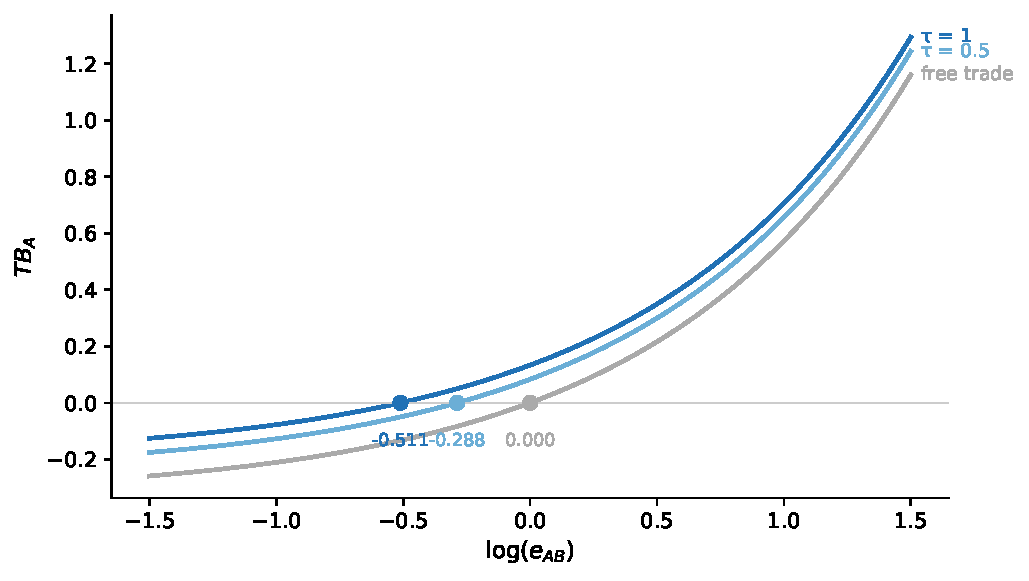
\includegraphics[width=0.8\textwidth]{2c2s1f_with_tariffs_eq.pdf}
    \caption{Trade balance deviation as a function of the exchange rate in the two-country model with tariffs. Equilibrium occurs where the trade balance deviation crosses zero. The figure is constructed under $A_{N_i}=A_{T_i}=1$, $\alpha_{T_i}=\alpha_N=1/3$, and the normalization $P_{T_A}=P_{T_B}=1$. In this calibration, the free-trade equilibrium exchange rate is $e=1$, and higher tariff rates lead to a larger equilibrium exchange rate appreciation.}
    \label{fig:2c2s1f_with_tariffs_eq}
\end{figure}
Substituting \eqref{eq:income_tariff} and the demand expressions into the trade balance condition $\mathrm{TB}_A = 0$ and solving for $e$ yields
\begin{equation}
e(\tau)
= \frac{1}{1+\tau}
\cdot \frac{1}{1 - \dfrac{\alpha_{T_B}\,\tau}{1+\tau}}
\cdot \frac{\alpha_{T_B}}{\alpha_{T_A}}
\cdot \frac{A_{T_A} L_A}{A_{T_B} L_B},
\label{eq:e_tau}
\end{equation}
which is strictly decreasing in $\tau$ for $\alpha_{T_B} > 0$. An increase in tariffs by country $A$ therefore requires an appreciation of its currency relative to country $B$ in equilibrium in order to offset the tariff-induced improvement in the trade balance at a given exchange rate.

\subsection{Robustness of the Two-Country Conventional Wisdom}
\label{sec:robustness}

The closed-form result in \rev{Section~\ref{sec:twocountry_cw}} relies on Cobb--Douglas preferences and linear production technologies. We now show that the qualitative prediction $de/d\tau < 0$ is independent of these assumptions: it follows from general monotonicity properties of import and export behavior\rev{. We state the monotonicity conditions as primitives and then note what they amount to: the exchange-rate condition of Lemma~\ref{lem:er_monotonicity} is the Marshall--Lerner condition, and the tariff condition of Lemma~\ref{lem:tariff_monotonicity} is its tariff analogue --- import expenditures falling in the consumer import price. The honest summary of this subsection is therefore that \emph{the conventional appreciation result holds wherever Marshall--Lerner holds}. This framing is deliberate, because it sets up the central point of Section~\ref{sec:threecountry}: bilateral Marshall--Lerner conditions do not pin down the sign of the multilateral exchange-rate response.} To establish this, we avoid solving each alternative specification in closed form and instead derive the sign of $de/d\tau$ from primitive conditions on trade flows. Equilibrium is characterized by balanced trade for country $A$,
\[
\mathrm{TB}_A(e,\tau) \equiv X_A(e,\tau) - M_A(e,\tau) = 0,
\]
where $e$ denotes units of country $A$'s currency per unit of country $B$'s currency and $\tau$ is an ad valorem tariff imposed by country $A$ on imports from country $B$. Assume that $\mathrm{TB}_A(e,\tau)$ is continuously differentiable and that $\mathrm{TB}_{A,e}(e,\tau) \neq 0$ locally. By the implicit function theorem, there exists a locally unique equilibrium mapping $e(\tau)$ satisfying
\[
\frac{de(\tau)}{d\tau} = -\frac{\mathrm{TB}_{A,\tau}(e(\tau),\tau)}{\mathrm{TB}_{A,e}(e(\tau),\tau)}.
\]
Thus, $de/d\tau < 0$ follows if $\mathrm{TB}_{A,\tau}(e,\tau) > 0$ and $\mathrm{TB}_{A,e}(e,\tau) > 0$ at equilibrium. Throughout, let $X_A(e,\tau)$ and $M_A(e,\tau)$ denote the values of exports and imports measured in country $A$'s currency. Let $p_M(e,\tau)$ denote the consumer price in country $A$ of imports from country $B$, and let $p_X(e)$ denote the price of country $A$'s exports faced by consumers in country $B$, expressed in $B$'s currency. Under the producer-price normalization $P_{T_A} = P_{T_B} = 1$,
\[
p_M(e,\tau) = (1+\tau)e, \qquad p_X(e) = \frac{1}{e}.
\]

\begin{lemma}[Tariff monotonicity]\label{lem:tariff_monotonicity}
Fix $e$. Suppose (i) the consumer import price $p_M(e,\tau)$ is increasing in $\tau$, and (ii) import expenditures $M_A(e,\tau)$ are decreasing in the consumer import price. In addition, suppose that any induced effect of $\tau$ on export revenues satisfies
\[
X_{A,\tau}(e,\tau) \ge 0\rev{, \qquad \text{or, under the weaker sufficient condition,} \qquad X_{A,\tau}(e,\tau) > M_{A,\tau}(e,\tau),}
\]
\rev{which permits export revenues to fall so long as they fall by less than import expenditures.} Then $\mathrm{TB}_{A,\tau}(e,\tau) > 0$.
\end{lemma}

\begin{proof}
Differentiating $\mathrm{TB}_A(e,\tau) = X_A(e,\tau) - M_A(e,\tau)$ with respect to $\tau$ at fixed $e$ yields $\mathrm{TB}_{A,\tau}(e,\tau) = X_{A,\tau}(e,\tau) - M_{A,\tau}(e,\tau)$. By (i)--(ii), $M_{A,\tau}(e,\tau) = (\partial M_A/\partial p_M)(\partial p_M/\partial\tau) < 0$. The stated condition on $X_{A,\tau}$ then implies $\mathrm{TB}_{A,\tau}(e,\tau) > 0$.
\end{proof}

\begin{remark}
In the baseline two-country model, the tariff applies only to imports and there is no policy response abroad, so $X_A(e,\tau)$ is independent of $\tau$ at fixed $e$. Hence $X_{A,\tau}(e,\tau) = 0$ and the condition of Lemma~\ref{lem:tariff_monotonicity} holds trivially.
\end{remark}

\begin{lemma}[Exchange-rate monotonicity]\label{lem:er_monotonicity}
Fix $\tau$. Suppose that a depreciation of country $A$'s currency (an increase in $e$) weakly improves its trade balance, in the sense that
\[
M_{A,e}(e,\tau) < 0 \qquad \text{and} \qquad X_{A,e}(e,\tau) \ge 0,
\]
with at least one inequality strict. Then $\mathrm{TB}_{A,e}(e,\tau) > 0$.
\end{lemma}

\begin{proof}
Differentiating $\mathrm{TB}_A(e,\tau) = X_A(e,\tau) - M_A(e,\tau)$ with respect to $e$ at fixed $\tau$ yields $\mathrm{TB}_{A,e}(e,\tau) = X_{A,e}(e,\tau) - M_{A,e}(e,\tau)$. Under the stated conditions, $-M_{A,e}(e,\tau) > 0$ and $X_{A,e}(e,\tau) \ge 0$, with at least one strict inequality, implying $\mathrm{TB}_{A,e}(e,\tau) > 0$.
\end{proof}

\begin{proposition}[Sign of exchange rate response to tariffs]\label{prop:sign_de_dtau}
Suppose that $\mathrm{TB}_A(e,\tau)$ is continuously differentiable and that $\mathrm{TB}_{A,e}(e,\tau) \neq 0$ in a neighborhood of an equilibrium $(e^*,\tau)$ satisfying $\mathrm{TB}_A(e^*,\tau) = 0$. If the conditions of Lemmas~\ref{lem:tariff_monotonicity} and~\ref{lem:er_monotonicity} hold in that neighborhood, then the equilibrium mapping $e(\tau)$ exists locally and satisfies $de(\tau)/d\tau < 0$.
\end{proposition}

\begin{proof}
By the implicit function theorem, there exists a locally unique function $e(\tau)$ such that $\mathrm{TB}_A(e(\tau),\tau) = 0$, and $de(\tau)/d\tau = -\mathrm{TB}_{A,\tau}(e(\tau),\tau)/\mathrm{TB}_{A,e}(e(\tau),\tau)$. Lemma~\ref{lem:tariff_monotonicity} implies $\mathrm{TB}_{A,\tau}(e,\tau) > 0$ and Lemma~\ref{lem:er_monotonicity} implies $\mathrm{TB}_{A,e}(e,\tau) > 0$, so $de(\tau)/d\tau < 0$.
\end{proof}

\rev{Lemmas~\ref{lem:tariff_monotonicity} and~\ref{lem:er_monotonicity} are satisfied under standard alternative preference, technology, and fiscal specifications precisely because those alternatives preserve the Marshall--Lerner logic; the supporting arguments are deferred to Appendix~\ref{app:robustness}. We emphasize the correct reading of this robustness: it is not that the appreciation result holds across ``a wide class of models'' in any unconditional sense, but that it holds wherever the bilateral Marshall--Lerner condition holds. In the two-country world, that condition is essentially the only economics in play. The next section shows that in a three-country world it is no longer sufficient: every bilateral Marshall--Lerner condition can hold and the multilateral response can still go either way, depending on substitution patterns \emph{across} foreign suppliers that the two-country model cannot express.}

\begin{revblock}
\subsection{The Exchange Rate as a Relative Wage}
\label{sec:relwage}

Before moving to three countries, it is worth stating explicitly what the exchange rate \emph{is} in this class of models, both to pre-empt confusion and to situate our contribution. The model is real and has no nominal anchor: money appears nowhere, and $e$ is determined by a balanced-trade condition, not by a monetary equilibrium. Under the producer-price normalization $P_{T_i} = 1$ in each country's own currency, competitive pricing implies $w_i = A_{T_i}$ in own-currency units, so
\[
\frac{\text{$B$'s wage in $A$'s currency}}{\text{$A$'s wage}} \;=\; \frac{e\, A_{T_B}}{A_{T_A}} \;\propto\; e .
\]
The nominal exchange rate is, up to a constant, the \emph{common-currency relative wage}; and because producer prices equal unit labor costs, it is simultaneously the terms of trade. All three objects coincide because there is one factor, constant returns, balanced trade, and no nominal rigidity. Statements below about ``depreciation of $A$'s currency'' are therefore statements about $A$'s relative wage and terms of trade, interpretable as long-run outcomes once prices have adjusted.

This object is familiar, and the connection runs deeper than analogy. An isolated tariff by $A$ on $B$, with $\tau_{AC}$ held at zero, is \emph{formally} a preferential arrangement in favor of $C$: up to the level of the external tariff and the treatment of revenue, raising $\tau_{AB}$ and cutting $\tau_{AC}$ are the same discriminatory wedge. The third-country consequences of that wedge are what the preferential-trade-agreement literature has tracked since \cite{viner1950}: \cite{mundell1964} on tariff preferences and the terms of trade, \cite{kempwan1976} on welfare-neutralizing external adjustments, the terms-of-trade externality framework of \cite{bagwell1999} and \cite{bagwell2002}, and, empirically, the excluded-country price effects of Mercosur measured by \cite{changwinters2002}. That literature's object of interest is welfare, but the mechanism it tracks --- the intermediate object in nearly every proposition --- is the bilateral terms of trade, which in the present model class \emph{is} the exchange rate. On the quantitative side, \cite{caliendo2015}, \cite{ossa2014}, and \cite{costinot2014} solve for exactly these relative-wage responses to arbitrary tariff vectors in many-country settings, and \cite{fajgelbaum2024trade} document the reallocation of trade toward untariffed origins empirically. What that literature does not provide, and what we add, is (i) a closed-form characterization of the \emph{sign} of the third-country relative-wage response to a discriminatory tariff, and of its dependence on the elasticity structure, home bias, relative size, and tariff magnitude; (ii) an impossibility result showing that under a single common elasticity the conventional two-country sign survives multilateralization as a theorem --- which we suggest is why the point has been overlooked; and (iii) the translation into exchange-rate language: the quantitative trade literature reports wage and welfare responses, but does not remark that its own equilibrium object implies that ``the dollar should depreciate against the euro'' is a possible consequence of a purely real tariff shock --- the inferential step at issue in the 2025 attribution debate.

\subsection{Scope and Modelling Choices}
\label{sec:scope}

Each restriction in the framework below is chosen for a purpose, and we state the purposes here rather than confessing the restrictions as limitations afterward.

\paragraph{The long run.} The paper characterizes the exchange rate consistent with a stationary external position, once prices have adjusted. This rules out nominal rigidities, which govern the \emph{speed} of adjustment, and portfolio flows, which govern \emph{deviations} during the transition --- neither of which changes what the trade channel alone eventually requires. Balanced trade is the zero-net-foreign-assets normalization of the intertemporal budget constraint. That normalization is not innocuous for the threshold's \emph{location}: solving the model with permanent trade imbalances $\mathrm{TB}_i = -b_i$, a US-scale deficit of $3$ percent of income raises the symmetric-point threshold from $3.96$ to between $4.6$ and $5.1$ depending on the counterpart of the deficit, while a surplus lowers it. What is invariant is the \emph{structure}: by the general-baseline result of Appendix~\ref{app:threshold}, reversal occurs if and only if $\rho$ exceeds a threshold determined by baseline shares and incomes, at any external position --- imbalances move the bar, not the logic. At 2025-scale tariffs, the tariff-size effect (which lowers the bar) dominates the deficit effect: the all-in threshold at $\tau = 1.45$ and a $3$ percent deficit is approximately $3.5$ for the real rate.

\paragraph{One factor.} A single mobile factor is a separate choice with a separate purpose, not a consequence of the long-run focus. It is what makes producer prices unit labor costs, hence makes the terms of trade \emph{equal} the relative wage rather than merely comove with it --- and that exactness is what licenses translating trade-theoretic results into exchange-rate language at all. Section~\ref{sec:rv} relaxes it (sector-specific factors) and shows the sign results are, if anything, strengthened.

\paragraph{No capital.} Domestic capital accumulation affects transition dynamics and shifts steady states --- second-order concerns for a long-run sign result, and the province of the dynamic quantitative literature \citep{eaton2016, caliendo2019}. An international \emph{financial account} is a different and deeper departure: it does not shift the balanced-trade condition, it replaces it with an intertemporal one. That model answers different questions; ours characterizes what trade flows alone pin down.

\paragraph{Three countries.} The country count faces a trilemma. Symmetric $n$-bloc models \citep{krugman1991, bond1996, yi2000} keep closed forms by removing exactly the heterogeneity the 2025 episode requires --- one cannot ask what happens when one bystander is small and highly substitutable while another is large and diversified. Quantitative many-country models \citep{caliendo2015, ossa2014} keep the heterogeneity at the cost of propositions. Three countries is the smallest number at which discrimination is possible at all --- a tariffed and an untariffed foreign partner --- and the largest at which sign conditions remain analytically available: the linearized system's numerator is a polynomial of degree $n-1$ in $\rho$, so $n = 3$ delivers a quadratic with a single economically relevant root, while at $n = 4$ single-crossing is no longer guaranteed even numerically.\footnote{This is not merely a worry about messy algebra: in four-country experiments we find asymmetric configurations in which the sign of $d\log e_{AC}/d\tau$ changes \emph{twice} as $\rho$ rises, so no single threshold exists to state.} The cost of the choice is stated plainly: with a single untariffed aggregate, the model cannot represent simultaneous appreciation against some bystanders and depreciation against others --- which is what the 2025 cross-section of bilateral rates in fact shows. The natural follow-up is to use the threshold of Proposition~\ref{prop:threshold}, in its general-baseline form, as a pair-by-pair diagnostic inside a calibrated many-country model.
\end{revblock}

\section{The Three-Country Model}
\label{sec:threecountry}

This section develops a three-country extension of the baseline framework and uses it to study how exchange rates adjust to tariffs when trade is multilateral. \rev{The Marshall--Lerner robustness established in Section~\ref{sec:robustness} sharpens what follows: every result below obtains in a model in which each bilateral Marshall--Lerner condition holds, so nothing that follows can be attributed to a failure of the two-country logic on its own terms. The question is what that logic leaves undetermined once a third country is present --- and the answer, it turns out, depends on a distinction between substitution margins that the two-country model has no way to express.}

\subsection{Model Setup}

We develop a static three-country model with CES preferences over differentiated tradable goods and flexible exchange rates, which allows us to isolate the role of substitution patterns across foreign suppliers.

\subsubsection{Firms}

Each country $i \in \{A,B,C\}$ produces one distinct tradable good $T_i$ and one non-tradable good $N_i$ using labor as the sole factor of production. Technologies are linear:
\begin{equation}
Y_{T_i} = A_{T_i} L_{T_i}, \qquad Y_{N_i} = A_{N_i} L_{N_i}, \qquad L_{T_i} + L_{N_i} = L_i,
\end{equation}
where $A_{T_i}$ and $A_{N_i}$ denote sectoral productivities and $L_i$ is the labor endowment in country $i$. Markets are perfectly competitive. As in the two-country model, we normalize the producer price of each tradable good to one, $P_{T_i} = 1$, and maintain this normalization throughout. Under linear technologies and perfect competition, firms earn zero profits and wages are equalized across sectors within each country. Equilibrium wages therefore satisfy $w_i = A_{T_i}$, with nontradable prices pinned down by $P_{N_i} = A_{T_i}/A_{N_i}$, exactly as in the two-country model.

\subsubsection{Households and Tariffs}

Households in each country $i \in \{A,B,C\}$ consume all three tradable goods and a locally produced non-tradable good. Preferences are nested: households allocate income between a tradable bundle and a non-tradable good via Cobb--Douglas, and substitute across tradable varieties via a CES aggregator:
\[
C_i = C_{T_i}^{\alpha_T}\, C_{N_i}^{\alpha_N}, \qquad C_{T_i} = \left[ \sum_{j \in \{A,B,C\}} \alpha_{T_j}^{1/\sigma} C_{T_j i}^{\frac{\sigma-1}{\sigma}} \right]^{\frac{\sigma}{\sigma-1}},
\]
where $\alpha_T = \alpha_{T_A} + \alpha_{T_B} + \alpha_{T_C}$, $\alpha_N = 1 - \alpha_T$, $\alpha_{T_j} > 0$, and $\sigma > 0$ is the elasticity of substitution across tradable varieties. The outer Cobb--Douglas layer fixes the expenditure share on the tradable bundle at $\alpha_T$ regardless of relative prices; the inner CES aggregator governs substitution across country varieties of tradables. Preference parameters are assumed to be identical across countries. The Cobb--Douglas model of Section~\ref{sec:twocountry} arises as the special case $\sigma = 1$, under which the inner CES collapses to Cobb--Douglas across all four goods.

Let $e_{ij}$ denote the nominal exchange rate defined as units of country $i$'s currency per unit of country $j$'s currency, with $e_{ii} = 1$ and the no-arbitrage condition $e_{ij} = e_{ik} e_{kj}$. In the three-country model the full exchange rate matrix is determined by two free bilateral rates, which we take to be $e_{AB}$ and $e_{AC}$; all other rates follow from no-arbitrage. Country $i$ applies an ad valorem tariff $\tau_{ij} \ge 0$ to consumption of tradable good $T_j$. Under the producer-price normalization $P_{T_j} = 1$, the consumer price of $T_j$ in country $i$ is $(1+\tau_{ij})e_{ij}$, with the tariff wedge $\tau_{ij} e_{ij}$ collected as government revenue and rebated lump-sum to households. The household budget constraint is
\begin{equation}
w_i L_i + T_i^{\mathrm{rev}} = \sum_{j \in \{A,B,C\}} (1+\tau_{ij})\, e_{ij}\, C_{T_j i} + P_{N_i}\, C_{N_i},
\label{eq:hh_budget_ces}
\end{equation}
where $T_i^{\mathrm{rev}} = \sum_{j} \tau_{ij} e_{ij} C_{T_j i}$. Letting $I_i = w_i L_i + T_i^{\mathrm{rev}}$ denote disposable income, the outer Cobb--Douglas layer allocates a fixed share $\alpha_T$ of income to the tradable bundle, and the inner CES demand gives
\begin{align}
C_{T_j i} &= \rev{\frac{\alpha_{T_j} \bigl((1+\tau_{ij})e_{ij}\bigr)^{-\sigma}}{\sum_{k} \alpha_{T_k} \bigl((1+\tau_{ik})e_{ik}\bigr)^{1-\sigma}}}\, \alpha_T\, I_i, \label{eq:ces_tradable_demand} \\[4pt]
C_{N_i} &= \frac{\alpha_N\, I_i}{P_{N_i}}. \label{eq:ces_nontradable_demand}
\end{align}
\rev{With the utility weights entering as $\alpha_{T_j}^{1/\sigma}$, the weights $\alpha_{T_j}$ are themselves the expenditure shares at unit relative prices, which is the convention we maintain throughout and the one used in the calibration.} The CES price index for the tradable bundle and the aggregate price level are
\begin{equation}
P_{T_i} = \left[ \sum_{j \in \{A,B,C\}} \rev{\frac{\alpha_{T_j}}{\alpha_T}} \bigl((1+\tau_{ij})e_{ij}\bigr)^{1-\sigma} \right]^{\frac{1}{1-\sigma}}, \qquad P_i = P_{T_i}^{\alpha_T}\, P_{N_i}^{\alpha_N},
\label{eq:price_level_ces}
\end{equation}
and the bilateral real exchange rate between countries $i$ and $j$ is $q_{ij} \equiv e_{ij} P_j / P_i$. \rev{The outer Cobb--Douglas layer fixes total tradable expenditure at $\alpha_T I_i$, but for $\sigma \neq 1$ the division of that budget across varieties depends on relative prices. Let
\begin{equation}
\varsigma_{ij} \;\equiv\; \alpha_T\, \frac{\alpha_{T_j} \bigl((1+\tau_{ij})e_{ij}\bigr)^{1-\sigma}}{\sum_{k} \alpha_{T_k} \bigl((1+\tau_{ik})e_{ik}\bigr)^{1-\sigma}}
\label{eq:realized_shares}
\end{equation}
denote the realized share of total income that country $i$ spends on variety $j$ (inclusive of tariffs), with $\sum_j \varsigma_{ij} = \alpha_T$. Substituting the demand expressions into the tariff revenue formula and solving for $I_i$ yields
\begin{equation}
I_i = \frac{w_i L_i}{1 - \displaystyle\sum_{j \in \{A,B,C\}} \varsigma_{ij}\, \dfrac{\tau_{ij}}{1+\tau_{ij}}},
\label{eq:income_ces}
\end{equation}
which remains a closed form because the shares $\varsigma_{ij}$ depend only on prices, not on income. At $\sigma = 1$ the realized shares collapse to the constants $\varsigma_{ij} = \alpha_{T_j}$ and \eqref{eq:income_ces} reduces to the natural generalization of the two-country income formula \eqref{eq:income_tariff}; for $\sigma \neq 1$, using the raw weights $\alpha_{T_j}$ in place of $\varsigma_{ij}$ mismeasures tariff revenue.\footnote{\rev{This distinction is quantitatively consequential: an earlier version of this paper used the fixed-weight formula for all $\sigma$, which overstated rebated revenue on tariffed imports at high $\sigma$ and generated a spurious sign reversal in $e_{AC}$. All results reported here use \eqref{eq:realized_shares}--\eqref{eq:income_ces}.}} Under free trade all $\tau_{ij} = 0$ and $I_i = w_i L_i$, while positive tariffs raise disposable income above wage income through the rebated revenue.}

\subsubsection{Market Clearing and Equilibrium}
\label{sec:equilibrium}

For each country $i \in \{A,B,C\}$, non-tradable goods are produced and consumed domestically. Market clearing requires $Y_{N_i} = C_{N_i}$, which using $Y_{N_i} = A_{N_i} L_{N_i}$, $P_{N_i} = w_i/A_{N_i}$, and \rev{the Cobb--Douglas outer layer ($P_{N_i} C_{N_i} = \alpha_N I_i$)} gives equilibrium labor allocations
\begin{equation}
\rev{\frac{L_{N_i}}{L_i} = \alpha_N\, \frac{I_i}{w_i L_i}}, \qquad \frac{L_{T_i}}{L_i} = 1 - \frac{L_{N_i}}{L_i},
\end{equation}
\rev{which equals $\alpha_N$ under free trade and exceeds it when rebated tariff revenue raises $I_i$ above wage income.} Each tradable variety $T_i$ is produced only in country $i$ and consumed in all countries. World market clearing for tradable $T_i$ requires $Y_{T_i} = \sum_{k} C_{T_i k}$, which using $Y_{T_i} = A_{T_i} L_{T_i}$ and \eqref{eq:ces_tradable_demand} gives
\begin{equation}
A_{T_i} L_{T_i} = \sum_{k \in \{A,B,C\}} \rev{\alpha_T\, I_k\, \frac{\alpha_{T_i} \bigl((1+\tau_{ki})e_{ki}\bigr)^{-\sigma}}{D_k}}, \qquad i \in \{A,B,C\},
\label{eq:tradable_market_clearing_ces}
\end{equation}
where \rev{$D_k = \sum_{m} \alpha_{T_m} \bigl((1+\tau_{km})e_{km}\bigr)^{1-\sigma}$ is the within-tradables CES denominator for country $k$; the non-tradable good does not enter $D_k$ because the outer Cobb--Douglas layer fixes its expenditure share at $\alpha_N$.} Note that $I_k$ here is the full disposable income from \eqref{eq:income_ces}, which already incorporates tariff revenue. Trade balances are measured in each country's own currency. \rev{Exports of $T_i$ from country $i$ to country $k$ are valued at the producer price in $i$'s own currency, $P_{T_i} C_{T_i k} = C_{T_i k}$,} while imports of $T_j$ into country $i$ are valued at $e_{ij} C_{T_j i}$\rev{, the producer-price value in $i$'s currency (the tariff wedge is a domestic transfer, not a payment abroad)}. The trade balance for country $i$ is therefore
\begin{equation}
\mathrm{TB}_i = \sum_{k \neq i} \rev{C_{T_i k}} - \sum_{j \neq i} e_{ij}\, C_{T_j i}, \qquad i \in \{A,B,C\}.
\label{eq:tb_ces_def}
\end{equation}
An equilibrium is a pair of nominal exchange rates $\{e_{AB}, e_{AC}\}$ such that $\mathrm{TB}_i = 0$ for all $i$. With three countries, only two of the three trade-balance conditions are independent by Walras' Law, so the system \eqref{eq:tb_ces_def} evaluated at $i \in \{B, C\}$ pins down the two free exchange rates, with $\mathrm{TB}_A = 0$ following automatically. All remaining exchange rates are recovered via no-arbitrage: $e_{BA} = 1/e_{AB}$, $e_{CA} = 1/e_{AC}$, and $e_{BC} = e_{AC}/e_{AB}$.

\subsubsection{Equilibrium Visualization}

\rev{Panel (a) of Figure~\ref{fig:loci}} illustrates equilibrium determination in a symmetric baseline calibration under Cobb-Douglas preferences ($\sigma = 1$), with $A_{T_i} = A_{N_i} = 1$ and $\alpha_{T_A} = \alpha_{T_B} = \alpha_{T_C} = \alpha_N = 1/4$. \rev{The panel} plots, in $(e_{AB}, e_{AC})$ space, the loci of exchange rates that satisfy $\mathrm{TB}_B = 0$ and $\mathrm{TB}_C = 0$. By symmetry, the two loci are mirror images around the 45-degree line and intersect at $e_{AB} = e_{AC} = 1$. The bottom-left region corresponds to combinations of $(e_{AB}, e_{AC})$ for which both $B$ and $C$ run trade surpluses against $A$, reflecting an overvaluation of $A$'s currency relative to both foreign currencies; the top-right region corresponds to the reverse. The remaining two quadrants feature offsetting imbalances, with one foreign country in surplus and the other in deficit.
\rev{Figure~\ref{fig:loci} collects the balanced-trade loci for the free-trade benchmark and for each of the three tariff experiments that follow in a single display.}
\begin{figure}[htbp]
    \centering
    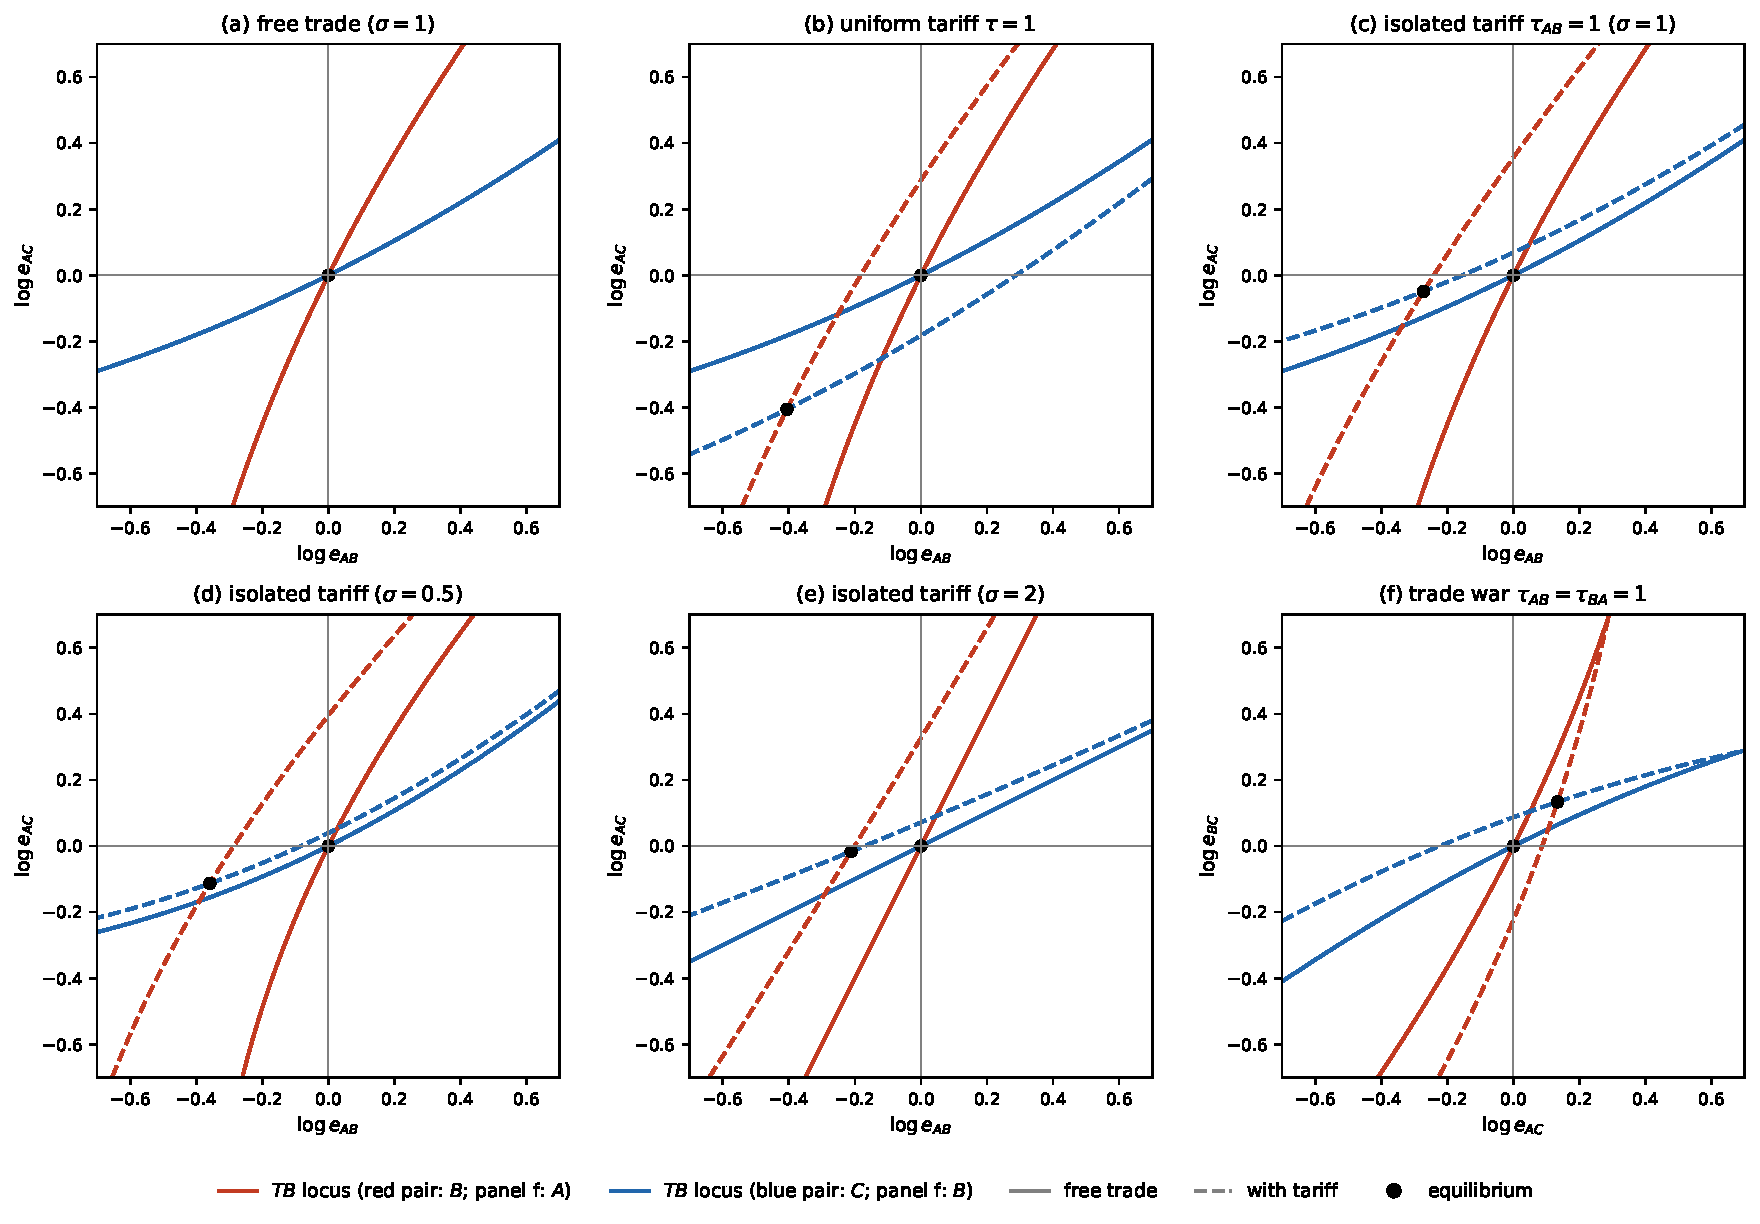
\includegraphics[width=\textwidth]{loci_multipanel.pdf}
    \caption{\rev{Balanced-trade loci and equilibria across the tariff experiments (symmetric baseline, $A_{T_i}=A_{N_i}=1$, $\alpha_{T_i}=\alpha_N=1/4$). Panels (a)--(e) plot the $\mathrm{TB}_B = 0$ (red) and $\mathrm{TB}_C = 0$ (blue) loci in $(\log e_{AB}, \log e_{AC})$ space; panel (f) plots the $\mathrm{TB}_A = 0$ (red) and $\mathrm{TB}_B = 0$ (blue) loci in $(\log e_{AC}, \log e_{BC})$ space. Solid: free trade; dashed: with the indicated tariff; dots: equilibria. (a) free trade; (b) uniform tariff $\tau = 1$; (c)--(e) isolated tariff $\tau_{AB} = 1$ at $\sigma = 1, 0.5, 2$; (f) trade war $\tau_{AB} = \tau_{BA} = 1$.}}
    \label{fig:loci}
\end{figure}

\subsection{Tariff Experiments}

This section studies the exchange rate response to tariffs in the three-country model. We consider three tariff configurations that progressively depart from the two-country benchmark: uniform tariffs, isolated tariffs, and bilateral trade war.

\subsubsection{Uniform Tariffs: The Two-Country Analogue}

We begin by considering a uniform tariff imposed by country $A$ on imports from both foreign countries, $B$ and $C$. Let $\tau \ge 0$ denote the common tariff applied to imports of both $T_B$ and $T_C$, so that $\tau_{AB} = \tau_{AC} = \tau$ and all other tariff rates are zero. With linear technologies and competitive firms, producer prices remain normalized at $P_{T_i} = 1$, wages satisfy $w_i = A_{T_i}$, and nontradable prices $P_{N_i} = A_{T_i}/A_{N_i}$ are unchanged. The tariff applies only to consumer prices in country $A$ and not to producer prices received abroad, so production decisions and sectoral labor allocations are unaffected. \rev{Panel (b) of Figure~\ref{fig:loci}} plots the trade-balance loci for countries $B$ and $C$ under free trade ($\tau = 0$, solid lines) and a uniform tariff ($\tau = 1$, dashed lines), under the symmetric baseline calibration $A_{T_i} = A_{N_i} = 1$ and $\alpha_{T_i} = \alpha_N = 1/4$.
Introducing a uniform tariff shifts both trade-balance loci outward relative to the 45-degree line, reflecting the reduction in import demand at any given exchange rate, and the new equilibrium corresponds to an appreciation of country $A$'s currency relative to both foreign currencies. Because the tariff is symmetric across foreign suppliers, country $A$'s currency appreciates by the same amount against $e_{AB}$ and $e_{AC}$. Changes in the elasticity of substitution affect the magnitude of the appreciation but not its sign. This configuration therefore provides the natural three-country analogue to the two-country benchmark: uniform tariffs replicate the conventional result unambiguously.

\subsubsection{Isolated Tariff: The Ambiguous Case}

We next consider an isolated tariff imposed by country $A$ on imports from country $B$ only, so that $\tau_{AB} = \tau > 0$ and $\tau_{AC} = 0$. This breaks symmetry across foreign suppliers and introduces an adjustment margin absent in the uniform-tariff case. \rev{Panel (c) of Figure~\ref{fig:loci}} plots the balanced-trade loci comparing free trade with an isolated tariff ($\tau_{AB} = 1$, dashed lines).
The tariff shifts country $B$'s balanced-trade locus outward, reflecting reduced access to $A$'s market, while country $C$'s locus shifts inward. As a result, $e_{AB}$ unambiguously falls — country $A$'s currency appreciates against $B$'s — whereas the sign of the response of $e_{AC}$ is \rev{not pinned down by the two-country logic} and depends on the relative magnitude of the two shifts. The ambiguity in $e_{AC}$ reflects two opposing general-equilibrium forces. The first is a trade-diversion effect: imports into $A$ are reallocated away from $B$ toward $C$, raising demand for $C$'s exports and putting appreciation pressure on $C$'s currency. The second is a trade-redirection effect: as $B$ loses access to $A$'s market, it reallocates exports toward $C$, increasing $C$'s imports and generating depreciation pressure on $C$'s currency. \rev{A third force operates alongside these two: the tariff also switches $A$'s expenditure toward $A$'s own goods --- the conventional two-country channel --- which strengthens $A$'s overall trade position and pushes toward appreciation against \emph{both} partners. Whether diversion can dominate is the central question of this section, and the answer under a single elasticity turns out to be an unambiguous no (Section~\ref{sec:impossibility}).}

When $\sigma$ is low, trade diversion is muted and the redirection channel dominates, so the equilibrium remains close to the two-country benchmark and country $A$'s currency \rev{appreciates substantially against $C$ as well as against $B$}.
\rev{Panel (d) of Figure~\ref{fig:loci}} illustrates this case for $\sigma = 0.5$\rev{: at the symmetric baseline with $\tau_{AB} = 1$, $\log e_{AC} = -0.11$. When $\sigma$ is higher, trade diversion toward country $C$ becomes quantitatively important and the appreciation of $A$ against $C$ shrinks: at $\sigma = 2$ (panel e) it has fallen to $\log e_{AC} = -0.016$, an order of magnitude smaller. The pattern is monotone --- as $\sigma$ grows, $\log e_{AC}$ rises toward zero \emph{from below}. It is tempting to extrapolate and conclude that at some sufficiently high $\sigma$ the sign flips and $A$ depreciates against $C$. It does not: Section~\ref{sec:impossibility} shows that under a single elasticity the response approaches zero asymptotically and never crosses, at this calibration for any $\sigma$ whatsoever. What the figures display is not a near-reversal but an asymptote.}
\rev{Country $A$'s tariff on $B$ generates an appreciation of $A$'s currency relative to $B$ at every elasticity, consistent with conventional intuition. The behavior of $e_{AC}$ is where the multilateral setting has something new to say --- but, as we show next, extracting it requires more than raising a single elasticity: it requires recognizing that ``substitution between $B$'s and $C$'s goods'' and ``substitution between home and imported goods'' are different margins, which the flat CES ties together by construction.}

\subsubsection{Bilateral Trade War: The Amplification Case}

Finally, we consider a bilateral trade war in which countries $A$ and $B$ impose reciprocal tariffs on one another, so that $\tau_{AB} = \tau_{BA} = \tau > 0$, while country $C$ remains untaxed. Relative to the isolated-tariff case, symmetry is restored between $A$ and $B$, which are now jointly engaged in tariff escalation from the perspective of the uninvolved third country. \rev{Panel (f) of Figure~\ref{fig:loci}} plots the balanced-trade loci for countries $A$ and $B$ in $(e_{AC}, e_{BC})$ space, comparing free trade (solid lines) with a bilateral trade war ($\tau_{AB} = \tau_{BA} = 1$, dashed lines).
The imposition of reciprocal tariffs shifts both countries' balanced-trade loci outward in $(e_{AC}, e_{BC})$ space. \rev{When $A$ and $B$ are of equal size and impose equal tariffs, the bilateral exchange rate $e_{AB}$ is unchanged by symmetry --- adjustment occurs entirely through a joint depreciation of both currencies relative to country $C$. We flag that this stability of $e_{AB}$ is a knife-edge property of the exactly symmetric configuration, not a general result: with $\tau_{AB} \neq \tau_{BA}$ or unequal country sizes, $e_{AB}$ moves, and in the calibration of Section~\ref{sec:calibration} it does. The joint depreciation against $C$, by contrast, is robust for near-symmetric wars. It is not unconditional: when one belligerent's tariff is far larger than the other's, the configuration approaches the isolated-tariff case and the dominant tariffer can appreciate mildly against $C$ even as its counterpart depreciates sharply; at 2025-scale bilateral rates ($\tau_{AB} = 1.45$, $\tau_{BA} = 1.25$) the war is comfortably inside the joint-depreciation region.

On magnitudes, a caution that previews Section~\ref{sec:impossibility}: within the single-elasticity specification, the size of the joint depreciation is \emph{decreasing} in $\sigma$ beyond low values, because a higher common elasticity also strengthens each belligerent's expenditure switching toward its own goods. It is the \emph{cross-origin} elasticity $\rho$ of the nested specification introduced below that governs the diversion force, and the joint depreciation is increasing in $\rho$ holding the home--import margin fixed. Conflating the two margins reverses the comparative static.

The configuration dependence delivered by the trade-war experiment --- appreciation against the tariffed partner under a unilateral tariff, multilateral depreciation under retaliation --- is exactly the pattern documented empirically by \cite{corsetti2025} in high-frequency responses to the 2018--20 and 2025 tariff announcements: the dollar appreciates when US tariffs are unilateral and depreciates when trading partners retaliate. In this model the pattern emerges from balanced-trade real adjustment alone.}

\begin{revblock}
\subsection{An Impossibility Result and a Reversal Threshold}
\label{sec:impossibility}

The experiments above left the sign of $e_{AC}$ to numerics. This subsection characterizes it analytically, and the characterization delivers the two central results of the paper. Throughout we work at the symmetric point --- equal sizes, common preferences, equal weights on the two foreign varieties --- and consider a marginal isolated tariff $d\tau$ imposed by $A$ on $B$; general baselines are treated at the end of the subsection and in Appendix~\ref{app:threshold}. Let $\alpha_D$ denote the home share of tradable expenditure and, as before, $\alpha_T$ the tradable share of total expenditure.

\paragraph{Impossibility under a common elasticity.} Consider first the flat specification of Section~\ref{sec:threecountry}, in which a single elasticity $\sigma$ governs substitution across all tradable varieties, with home expenditure share $\alpha_D$ within tradables.

\begin{proposition}[Impossibility]
\label{prop:impossibility}
In the single-elasticity model, the local response of the third-country exchange rate to an isolated tariff satisfies
\[
\left.\frac{d \log e_{AC}}{d\tau}\right|_{\tau=0}
= -\,\frac{\sigma\,(3\alpha_D - 1) + 3(1-\alpha_D)(1-\alpha_T)}{3\left[\,3\alpha_D(\sigma-1) + \sigma + 1\,\right]} .
\]
If $\alpha_D \ge 1/3$, the numerator is positive for every $\sigma > 0$: country $A$'s currency appreciates against the untariffed third country at any elasticity. At the symmetric baseline calibration ($\alpha_{T_j} = \alpha_N = 1/4$, so $\alpha_D = 1/3$, $\alpha_T = 3/4$), the response is exactly $-1/(12\sigma)$, which approaches zero from below as $\sigma \to \infty$ but never crosses it.
\end{proposition}

The proof is a special case of Proposition~\ref{prop:threshold} below (set $\rho = \eta = \sigma$). The economics is worth stating in words. A higher $\sigma$ does strengthen trade diversion --- $A$'s imports reallocate more elastically from $B$ toward $C$. But the same $\sigma$ governs substitution between imports and \emph{home} goods, so it strengthens conventional expenditure switching in exactly the same proportion. The bar that the diversion force must clear rises one-for-one with the force itself, and for any realistic home bias ($\alpha_D \ge 1/3$; actual economies' home shares of tradable expenditure are far higher) the race is unwinnable at every $\sigma$. Figure~\ref{fig:threshold} (panel a, dashed) displays the resulting asymptote. We verify numerically that the conclusion is not an artifact of the local approximation: across the full tariff grid ($\tau$ up to $1.5$) and $\sigma$ up to $50$, $\log e_{AC} \le 0$ at every point.\footnote{This impossibility result also explains, we believe, why the multilateral fragility of the two-country prediction has gone unnoticed: the natural first extension --- adding a third country to a one-elasticity CES model --- genuinely cannot produce it.}

\paragraph{Separating the margins.} The single elasticity is doing double duty. To separate the two margins, replace the flat tradable aggregator with the nested structure
\[
C_{T_i} = \left[ \alpha_D^{1/\eta}\, C_{T_i i}^{\frac{\eta-1}{\eta}} + (1-\alpha_D)^{1/\eta}\, M_i^{\frac{\eta-1}{\eta}} \right]^{\frac{\eta}{\eta-1}},
\qquad
M_i = \Bigg[ \sum_{j \neq i} \beta_j^{1/\rho}\, C_{T_j i}^{\frac{\rho-1}{\rho}} \Bigg]^{\frac{\rho}{\rho-1}},
\]
where $\eta$ is the macro (home-versus-import) Armington elasticity, $\rho$ is the micro (cross-origin) elasticity across foreign suppliers, and $\beta_j = 1/2$ at the symmetric point. The outer Cobb--Douglas layer over tradables and non-tradables is unchanged, and the flat model is the special case $\rho = \eta = \sigma$. The distinction between the two elasticities is not a modeling flourish: it is the wedge documented empirically by \cite{feenstra2018}, who find micro (cross-origin) elasticities substantially above macro (home--import) ones, with product-level dispersion in \cite{broda2006} and the China--Vietnam reallocation case in \cite{fajgelbaum2024trade}.

\begin{proposition}[Reversal threshold]
\label{prop:threshold}
In the nested model at the symmetric point,
\[
\left.\frac{d \log e_{AC}}{d\tau}\right|_{\tau=0}
= \frac{\rho - \rho^*}{3\left[\,3\alpha_D(\eta-1) + \rho + 1\,\right]},
\qquad
\boxed{\;\rho^* = 3\left[\,1 + \alpha_D(\eta - 1) - \alpha_T(1-\alpha_D)\,\right]\;}
\]
The denominator is positive whenever $\eta \ge 1$; this is the local stability condition for the balanced-trade equilibrium. Hence country $A$'s currency depreciates against the untariffed third country in response to a marginal discriminatory tariff on $B$ if and only if $\rho > \rho^*$.
\end{proposition}

The comparative statics of the threshold are all interpretable. $\rho^*$ is increasing in home bias $\alpha_D$ (a more home-biased $A$ has less import expenditure to divert; $\partial \rho^*/\partial \alpha_D = 3[(\eta-1)+\alpha_T] > 0$), increasing in the macro elasticity $\eta$ (stronger home--import switching raises the bar), and decreasing in the tradable share $\alpha_T$. \rev{Note the division of labor this implies between the two calibration corrections of this revision: realistic home bias is a \emph{credibility} fix --- it disciplines magnitudes and modestly raises the bar --- while the separation of the two elasticities is what makes the reversal possible at all; fixing home bias alone under a common elasticity leaves the impossibility result fully in force. A note on language is also worth one sentence, because everyday phrasing invites a mistake here: ``Chinese and Vietnamese goods are closer substitutes than American and Chinese goods'' sounds like bilateral heterogeneity across country pairs, but it is exactly the $\rho$-versus-$\eta$ distinction --- the first comparison is foreign-versus-foreign, the second home-versus-foreign --- and requires no bilateral elasticity matrix.} Quantitatively, at US-realistic parameters --- home bias $\alpha_D = 0.80$, tradable share $\alpha_T = 0.40$, macro elasticity $\eta = 1.5$ in the range of \cite{feenstra2018} --- the threshold is $\rho^* = 3.96$. Table~\ref{tab:rhostar_grid} reports the threshold across the empirically relevant parameter box: $\rho^*$ lies between roughly $2.5$ and $5.5$. \rev{Whether measured cross-origin elasticities clear the bar is episode-dependent, and we state the claim with its qualifications. Adjustments push in both directions: a US-scale trade deficit raises the threshold (Section~\ref{sec:scope}), the real-rate objective raises it (below), and tariff size lowers it. For 2025-scale tariffs the all-in threshold --- real rate, $3$ percent deficit, $\tau = 1.45$ --- is approximately $3.5$, inside the measured range with room; for marginal tariffs at a US-scale deficit it is $5$--$6.5$, attainable only at the upper end of the estimates.} The reversal is therefore not a knife-edge curiosity --- it is attainable at standard parameter values --- but it is \emph{invisible} to any specification that conflates the two margins. Figure~\ref{fig:threshold} summarizes both results.

\begin{figure}[htbp]
    \centering
    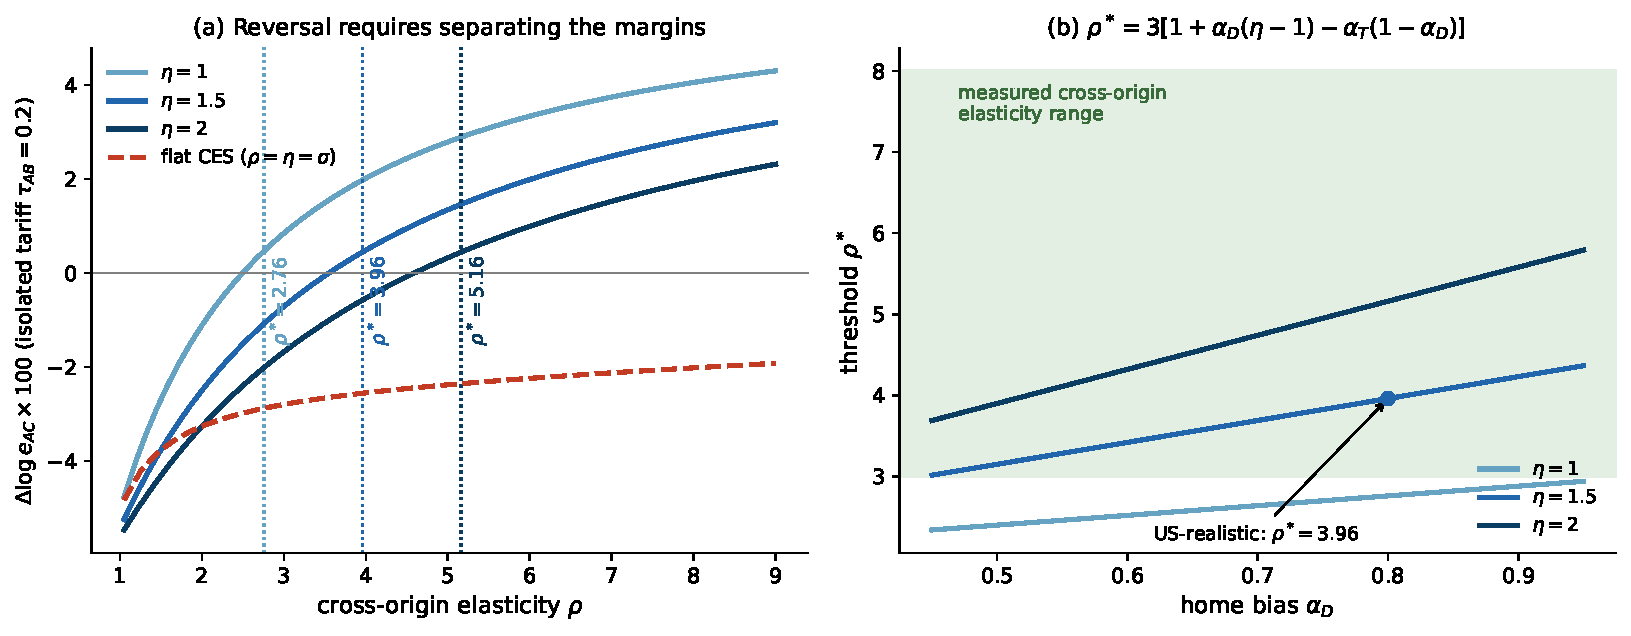
\includegraphics[width=\textwidth]{threshold_figure.pdf}
    \caption{The reversal threshold. Panel (a): equilibrium change in $\log e_{AC}$ following an isolated tariff $\tau_{AB} = 0.2$, as a function of the cross-origin elasticity $\rho$, for three values of the macro elasticity $\eta$ ($\alpha_D = 0.80$, $\alpha_T = 0.40$, equal sizes). Vertical dotted lines mark the analytic thresholds $\rho^*(\eta)$ of Proposition~\ref{prop:threshold}; each equilibrium path crosses zero slightly before its marked threshold because $\rho^*$ is the marginal ($\tau \to 0$) threshold and the threshold falls with the tariff. The dashed path imposes $\rho = \eta = \sigma$ (the flat CES): it approaches zero but never crosses --- Proposition~\ref{prop:impossibility}. Panel (b): the threshold as a function of home bias $\alpha_D$; the shaded band indicates the range of measured cross-origin elasticities.}
    \label{fig:threshold}
\end{figure}

\begin{table}[htbp]
\centering
\begin{tabular}{lccc@{\hspace{1.2cm}}lcc}
\hline\hline
\multicolumn{4}{l}{\textit{Panel A: $\rho^*$ by home bias and $\eta$ ($\alpha_T = 0.40$)}} & \multicolumn{3}{l}{\textit{Panel B: by third-country size / tariff}} \\[2pt]
 & $\eta = 1.0$ & $\eta = 1.5$ & $\eta = 2.0$ & & $L_C$ & $\rho^*$ \\
\cline{1-4}\cline{5-7}
$\alpha_D = 0.60$ & 2.52 & 3.42 & 4.32 & Vietnam & 0.055 & 8.76 \\
$\alpha_D = 0.70$ & 2.64 & 3.69 & 4.74 & EU & 0.86 & 4.32 \\
$\alpha_D = 0.80$ & 2.76 & 3.96 & 5.16 & equal & 1.00 & 4.24 \\
$\alpha_D = 0.85$ & 2.82 & 4.09 & 5.37 & ROW & 3.51 & 3.78 \\
$\alpha_D = 0.90$ & 2.88 & 4.23 & 5.58 & & $\tau$ & $\rho^*(\tau)$ \\
\cline{5-7}
 & & & & & 0.20 & 3.55 \\
 & & & & & 0.50 & 3.19 \\
 & & & & & 1.00 & 2.86 \\
 & & & & & 1.45 & 2.70 \\
\hline\hline
\end{tabular}
\caption{The reversal threshold $\rho^*$. Panel A: analytic threshold of Proposition~\ref{prop:threshold} over the empirically relevant $(\alpha_D, \eta)$ box. Panel B, top: numerical threshold by third-country size at $\alpha_D = 0.80$, $\alpha_T = 0.40$, $\eta = 1.5$, $L_B = 1.21$ (sizes as in the Section~\ref{sec:calibration} calibration). Panel B, bottom: the discrete-tariff threshold --- the $\rho$ at which the \emph{total} change in $\log e_{AC}$ over $[0, \tau]$ is zero --- at equal sizes; it falls monotonically with the tariff, so the local threshold is a conservative bound and 2025-scale tariffs make the reversal easier, not harder.}
\label{tab:rhostar_grid}
\end{table}

\paragraph{Third-country size.} Panel B of Table~\ref{tab:rhostar_grid} reports the threshold for unequal sizes, computed at the size configurations of the calibration in Section~\ref{sec:calibration}. The threshold is \emph{decreasing} in the size of the third country: a small $C$ cannot absorb diverted demand without a large wage response, so its currency appreciates sharply per unit of diverted expenditure and pushes $e_{AC}$ down. This has a sobering implication for where one should expect to observe the reversal. Vietnam --- often cited as the natural destination of trade diverted from China, and assigned the \emph{highest} substitution elasticity in our calibration --- faces by far the \emph{highest} threshold ($\rho^* = 8.76$): small, highly substitutable third countries are where the mechanism is hardest to see in bilateral rates, not easiest. Large aggregates such as the EU or the rest of the world, with thresholds near $4$, are the natural place to look.

\paragraph{Large tariffs.} Proposition~\ref{prop:threshold} is local. Since the 2025 episode involves tariffs above $100$ percent, Panel B also reports the discrete-tariff threshold: the value of $\rho$ at which the cumulative change in $\log e_{AC}$ over $[0,\tau]$ equals zero. It falls monotonically in $\tau$ --- from $3.96$ at $\tau \to 0$ to $2.70$ at $\tau = 1.45$ at equal sizes --- so the linearized threshold is a conservative upper bound, and the large tariffs of the 2025 episode make the reversal region strictly larger.

\paragraph{The real exchange rate.} The propositions are stated for $e$, which is the relative wage and the terms of trade; the CPI-based real rate $q_{AC} = e_{AC} P_C / P_A$ is a distinct object because the tariff enters $A$'s consumer price index directly. Since $P_{N_i} = A_{T_i}/A_{N_i}$ is a pure productivity ratio untouched by the tariff, all real-exchange-rate action runs through tradables --- the non-tradable sector is inert \emph{for the mechanism} but governs the mapping from $e$ to $q$. The mapping matters for the threshold: the tariff mechanically raises $A$'s tariff-inclusive price index, absorbing part of any nominal depreciation, so real depreciation against $C$ requires more diversion than nominal depreciation does. At the benchmark parameters the real-rate threshold is $\rho^*_q = 4.93$ against $\rho^* = 3.96$ for the nominal rate --- both inside the measured cross-origin range, with the gap equal to the tariff's direct CPI contribution. The calibration in Section~\ref{sec:calibration} reports both objects.

\paragraph{General baselines.} The symmetric-point formula generalizes. Linearizing the two balanced-trade conditions at an arbitrary free-trade baseline described by observables --- common-currency incomes $y_i$, home shares $h_i$ of tradable expenditure, and import-bundle origin shares $b_{ij}$ --- the local response takes the form $d\log e_{AC}/d\tau = N(\rho)/D$, where $N$ is a \emph{quadratic} in $\rho$ with leading coefficient $b_{AB}\, b_{AC}\, b_{CA}\, b_{CB}\, (1-h_A)(1-h_C)\, y_A\, y_C > 0$. The threshold at any baseline is therefore the larger root of $N$, and the qualitative statement --- depreciation against the untariffed third country if and only if $\rho$ exceeds a threshold --- holds for arbitrary sizes and asymmetric trade patterns, with the threshold expressed entirely in terms of baseline expenditure shares and incomes. Appendix~\ref{app:threshold} states the result and sketches the derivation; the symmetric point recovers Proposition~\ref{prop:threshold} exactly.
\end{revblock}

\subsection{Economic Mechanisms and Extensions}

The tariff experiments illustrate that the standard two-country intuition for exchange-rate adjustment need not extend to multilateral trade environments. In a three-country setting, an isolated tariff imposed by country $A$ on imports from $B$ generates opposing trade-diversion and trade-redirection forces\rev{, and Section~\ref{sec:impossibility} showed exactly when diversion wins: never under a common elasticity, and precisely when $\rho > \rho^*$ once the cross-origin and home--import margins are separated}. The bilateral trade war case resolves this ambiguity: when both $A$ and $B$ impose reciprocal tariffs, the two forces reinforce one another from $C$'s perspective, producing an unambiguous joint depreciation of $A$ and $B$ relative to $C$ \rev{for near-symmetric wars}.

The relative importance of the trade-diversion channel depends on several features that can be incorporated in richer models. First, \rev{as established above, the cross-origin elasticity $\rho$ between goods produced by $B$ and $C$ in $A$'s market is the central parameter, and it must be distinguished from the home--import elasticity $\eta$: raising a single common elasticity strengthens the diversion and expenditure-switching forces in lockstep and can never deliver the reversal (Proposition~\ref{prop:impossibility})}. Second, the strength of the diversion channel depends on expenditure patterns. When goods from country $C$ account for a large share of $A$'s import basket, relative price changes translate into larger demand reallocations toward $C$. Such asymmetries arise naturally from heterogeneous preference weights $\alpha_{T_j}$ across tradable varieties\rev{, and Appendix~\ref{app:threshold} shows how the threshold depends on them through baseline expenditure shares}. Third, supply-side considerations matter\rev{, and here the exchange-rate implication runs opposite to the quantity intuition. Capacity constraints or increasing marginal costs in country $C$ do limit the \emph{quantity} expansion of $C$'s exports --- but precisely for that reason they concentrate the incidence of diverted demand in $C$'s price, which under the producer-price normalization \emph{is} $C$'s currency. Upward-sloping export supply therefore strengthens, not dampens, the appreciation of $C$ per unit of diverted demand, and lowers the reversal threshold. We formalize this below with a sector-specific-factors extension.}

Finally, initial trade patterns may also shape the strength of the trade-redirection channel. When the elasticity of demand in country $C$ for goods from $B$ is low, or when $C$'s import capacity is limited, the redirection of $B$'s exports following the tariff has a muted effect on $C$'s import prices and hence on depreciation pressure on $C$'s currency. This mechanism is related to the trade deflection literature \citep{bown2007}, who document empirically that import restrictions by one country redirect exports toward third market. Larger tariff shocks amplify the expenditure-switching and trade-diversion channels by inducing larger reallocations of trade flows \citep{amiti2019}.

\begin{revblock}
\subsubsection{Sector-Specific Factors: Upward-Sloping Export Supply}
\label{sec:rv}

The linear technology makes export supply infinitely elastic at the going wage. To formalize the supply-side channel discussed above, we introduce a sector-specific fixed factor in tradables --- the Ricardo--Viner structure --- replacing $Y_{T_i} = A_{T_i} L_{T_i}$ with
\[
Y_{T_i} = A_{T_i} L_{T_i}^{\gamma}, \qquad \gamma \le 1,
\]
with non-tradables linear as before and labor mobile across sectors within each country. Competitive pricing gives $w_i = \gamma A_{T_i} L_{T_i}^{\gamma-1}$ under the producer-price normalization, with the fixed factor earning rents $(1-\gamma) P_{T_i} Y_{T_i}$ that are distributed lump-sum to households. The sectoral labor allocation becomes endogenous to the tariff, and $\gamma = 1$ recovers the baseline exactly. Equilibrium is a five-equation system --- non-tradable market clearing in each country plus two balanced-trade conditions --- solved numerically.

Two results, both in the direction anticipated by the discussion above. First, at the symmetric benchmark the reversal threshold falls with the degree of diminishing returns, though modestly: $\rho^*$ declines from $3.96$ at $\gamma = 1$ to $3.83$ at $\gamma = 0.5$. Second, and quantitatively more important, diminishing returns \emph{compress the size gradient} of the threshold. Upward-sloping export supply binds most for a small third country --- which cannot expand export quantities cheaply, so that diverted demand is absorbed by its price, i.e.\ its currency --- and this is exactly where the baseline mechanism was weakest:
\begin{center}
\begin{tabular}{lccc}
\hline
 & Vietnam ($L_C = 0.055$) & EU ($L_C = 0.86$) & ROW ($L_C = 3.51$) \\
\hline
$\gamma = 1$ (baseline) & 8.76 & 4.32 & 3.78 \\
$\gamma = 0.8$          & 6.07 & 4.18 & 3.78 \\
$\gamma = 2/3$          & 5.27 & 4.09 & 3.77 \\
\hline
\end{tabular}
\end{center}
Vietnam's threshold falls by forty percent while the large aggregates barely move. Sector-specific factors thus partially rehabilitate small, supply-constrained third countries as venues for the reversal, without changing any qualitative conclusion of Section~\ref{sec:impossibility}. We emphasize the converse implication as well: none of the sign results require diminishing returns --- the minimal linear structure delivers them, which is precisely why we use it as the baseline.

\paragraph{The boundary of the exercise.} Two literatures mark where the static framework stops being the right tool, and we state the boundary deliberately rather than as a caveat. Dynamic quantitative trade models with capital accumulation \citep{eaton2016, caliendo2019} supersede this framework on magnitudes and transition paths --- tariffs move investment demand, and the path differs from the steady state --- but not on the sign mechanism itself, which requires neither capital nor dynamics. Intertemporal open-economy analysis \citep{obstfeld1996foundations} adds a distinction the static model cannot express: a \emph{temporary} tariff and a \emph{permanent} tariff have different (and potentially opposite) exchange-rate implications once saving responds. Our static structure implicitly treats tariffs as permanent, a strong assumption in an episode whose defining feature was uncertainty about persistence \citep{kalemli2025}; the results are accordingly best read as characterizing the long-run position conditional on the tariffs persisting.
\end{revblock}

\section{Calibration Exercise}
\label{sec:calibration}

We calibrate the three-country model to offer quantitative guidance on the mechanisms identified in Section~\ref{sec:threecountry}, using the 2025 US reciprocal tariff episode as the application. In this episode, the United States imposed large tariffs on imports from a range of trading partners, with particularly high rates directed at China and China retaliating in kind, culminating in effective bilateral tariff rates exceeding 100 percent by mid-2025. We consider three alternative configurations for the third economy $C$: the European Union, representing a large bloc of advanced-economy trading partners with deep trade links to both the US and China; Vietnam, representing a smaller economy that has emerged as a significant node for trade redirection away from the direct US-China bilateral linkage; and the rest of the world aggregated as a single block.

The model is deliberately stylized, and the calibration exercise should be interpreted not as a realistic simulation of the episode but as an illustration of the relative importance of the trade-diversion and trade-redirection channels under parameter configurations that are broadly consistent with its observable features. The parameters we vary across configurations are the expenditure shares $\{\alpha_{T_A}, \alpha_{T_B}, \alpha_{T_C}, \alpha_N\}$, which govern bilateral trade intensities; the labor endowments $\{L_A, L_B, L_C\}$, which govern relative economic size; and the tariff rates $\{\tau_{AB}, \tau_{BA}\}$ for the trade war experiment or $\tau_{AB}$ alone for the isolated tariff case. We set productivity parameters to $A_{T_i} = A_{N_i} = 1$ for all economies, so that relative economic size is captured entirely through the endowments $L_i$.


\subsection{Tariff Regimes}
We consider two tariff regimes corresponding to distinct phases of the 2025 US-China trade conflict, measured as incremental tariff rates above the pre-2025 baseline. The US is country $A$, China is country $B$, and the third country $C$ varies across configurations. Table~\ref{tab:tariff_regimes} summarizes the tariff rates across both regimes and configurations; full details of the rate construction are provided in Appendix~\ref{app:tariffs}.

Regime 1 imposes a unilateral US tariff on China with no retaliation and no tariff on $C$, mapping directly onto the isolated tariff experiment of Section~\ref{sec:threecountry}. Regime 2 represents peak bilateral escalation between the US and China; the rates are not exactly symmetric but are of similar magnitude and map naturally onto the trade war experiment. Furthermore, regime 2 includes $\tau_{AC} = 0.10$ across all configurations in this regime, reflecting the universal baseline tariff that remained in place for non-China trading partners after the April 9 pause. \rev{Regime 3 collects the rates in force at our extended December 2025 comparison window, after the May Geneva truce and the November 10 fentanyl-tariff reduction: 20 percent on China (10 reciprocal plus 10 fentanyl), 10 percent Chinese retaliation, and the 2025 framework rates on third countries (15 percent for the EU, 20 percent for Vietnam, roughly 15 percent for the ROW aggregate). The methodological principle is that \emph{each data window is compared to the tariff vector actually in force in that window} --- a discipline that matters, because the December structure is nearly uniform across China and third countries, which switches the model's relevant experiment from the trade war to the uniform-tariff case. Where announced-but-paused rates differed sharply from in-force rates (the April 2 schedule: 20 percent on the EU, 46 percent on Vietnam), we report an announced-rate variant in the replication package.}

\begin{table}[htbp]
\centering
\begin{tabular}{llcccccc}
\hline
& & \multicolumn{2}{c}{US-China} & \multicolumn{2}{c}{US-$C$} & \multicolumn{2}{c}{$C$-US} \\
\cmidrule(lr){3-4}\cmidrule(lr){5-6}\cmidrule(lr){7-8}
Regime & Description & $\tau_{AB}$ & $\tau_{BA}$ & $\tau_{AC}^{\mathrm{EU}}$ & $\tau_{AC}^{\mathrm{VNM}}$ & $\tau_{CA}$ & Type \\
\hline
1 & Fentanyl-related tariffs        & 0.20 & 0.00 & 0.00 & 0.00 & 0.00 & Isolated \\
2 & Peak escalation                 & 1.45 & 1.25 & 0.10 & 0.10 & 0.00 & Trade war \\
\rev{3} & \rev{Late-2025 (post-truce)} & \rev{0.20} & \rev{0.10} & \rev{0.15} & \rev{0.20} & \rev{0.00} & \rev{Near-uniform} \\
\hline
\end{tabular}
\caption{Tariff regimes used in the calibration exercise. Rates are incremental ad valorem tariffs above the pre-2025 baseline. $\tau_{AB}$ is the US tariff on China, $\tau_{BA}$ is the Chinese tariff on the US, $\tau_{AC}$ is the US tariff on $C$, and $\tau_{CA}$ is $C$'s tariff on the US. The ROW configuration uses the same $\tau_{AC}$ as EU and Vietnam.}
\label{tab:tariff_regimes}
\end{table}

\subsection{Preference and Endowment Calibration}

\begin{revblock}
The calibration uses the nested demand system of Section~\ref{sec:impossibility} with \emph{country-specific} preferences calibrated from bilateral import shares in absorption --- not, as in an earlier version of this paper, common preferences from world export shares, which counterfactually implied that the US spends more on Chinese tradables than on its own. For each country $i$ in a configuration, the expenditure share on partner $j$'s goods is measured as 2024 goods imports from $j$ (importer-reported: US Census, China GACC, Eurostat, Vietnamese customs) divided by nominal GDP; the tradable expenditure share is $\alpha_T = 0.40$ throughout; the home tradable share $\alpha_{D_i}$ absorbs the residual, including goods from outside the trio (a conservative choice for the diversion mechanism); and the import-bundle weights $\beta_{ij}$ follow from the partner split. Preference weights are then \emph{inverted at the model's free-trade equilibrium} --- iterated until the equilibrium realized shares reproduce the data shares exactly --- since with unequal country sizes equilibrium prices differ from unity and weights are not shares. Labor endowments remain proportional to 2024 PPP GDP \citep{imf2024weo}, and $A_{T_i} = A_{N_i} = 1$. Table~\ref{tab:calibration} reports the implied home-bias parameters: US home bias is now $0.91$--$0.95$ across configurations, in line with the observation that US spending on Chinese goods is on the order of $1$--$2$ percent of expenditure.

A note on what ``home'' means in a trio. Within US tradable spending at border values, Chinese goods are $3.8$ percent, EU goods $5.2$ percent, and \emph{all} foreign goods $28$ percent. The high trio home shares ($0.89$--$0.95$) arise because goods from countries outside the trio must be assigned somewhere, and we assign them to home; the alternative of excluding non-trio imports from the basket entirely gives $\alpha_{D_A} = 0.89$ and moves the results by a few tenths of a percentage point. The genuinely lower home-bias world --- all foreign goods treated as the composite partner, $\alpha_{D_A} = 0.72$ --- \emph{is} the ROW configuration. The trio configurations therefore bracket the treatments of non-trio trade, and the results are insensitive to the bracketing.

\begin{table}[htbp]
\centering
\begin{tabular}{lcccccc}
\hline
Configuration & $\alpha_{D_A}$ & $\alpha_{D_B}$ & $\alpha_{D_C}$ & $s_{A,B}$ & $s_{A,C}$ & $L_C / L_A$ \\
\hline
US--China--EU  & 0.911 & 0.941 & 0.881 & 1.50\% & 2.08\% & 0.86 \\
US--China--Vietnam (adj.) & 0.951 & 0.969 & 0.553 & 1.50\% & 0.47\% & 0.055 \\
US--China--ROW & 0.720 & 0.647 & 0.803 & 1.50\% & 9.69\% & 3.51 \\
\hline
\end{tabular}
\caption{Import-share calibration by configuration. $\alpha_{D_i}$: country $i$'s home share of tradable expenditure implied by 2024 bilateral goods imports over nominal GDP ($\alpha_T = 0.40$); $s_{A,j}$: US expenditure share on partner $j$'s goods. The Vietnam configuration applies a processing-trade adjustment, treating half of Vietnam's gross imports from China as final absorption (unadjusted, Vietnam's gross imports from China are 30 percent of its GDP and its implied home share falls to $0.175$); both variants are reported in the replication package. Sources and construction details in the replication package (\texttt{calibration\_inputs.json}).}
\label{tab:calibration}
\end{table}

For the elasticities, we fix the macro (home--import) elasticity at $\eta = 1.5$, within the macro range of \cite{feenstra2018}, and report results over a \emph{grid} of cross-origin elasticities $\rho \in [1.5, 8]$ with each configuration's reversal thresholds marked, rather than assigning a single value per configuration. The empirically central range for $\rho$ is roughly $2$--$4$: median cross-origin estimates in \cite{broda2006} at three-digit aggregation lie near $2.5$--$4$, and \cite{liqiu2022} --- who estimate exactly the two-elasticity structure used here on bilateral trade, tariff, and production data --- find the home--foreign elasticity $43$ percent below the cross-foreign one, implying $\rho \approx 1.75\,\eta \approx 2.6$ at our $\eta$. Configuration-specific values of $\rho$ are legitimate in this design because each configuration is a self-contained three-country world: $\rho$ is the substitutability between \emph{that} pair of suppliers in \emph{that} aggregation, so the China--Vietnam elasticity may well exceed the China--ROW one \citep{fajgelbaum2024trade, fajgelbaum2020return} --- but this is now expressed by where each configuration sits on the reported grid rather than by a hand-assigned point value.\footnote{Appendix~\ref{app:extended_calibrations} retains six additional third-country configurations under the previous calibration for reference; their rebuild under the import-share approach requires additional bilateral data collection and is left to the replication package.}
\end{revblock}

\subsection{Results and Comparison With Data}

Figure~\ref{fig:results} reports model-implied Regime-2 exchange rate changes across the $\rho$ grid alongside realized data. The data refer to percent changes\footnote{We report $100 \times (\text{level}_t / \text{level}_0 - 1)$ relative to the 2024 annual average.} in observed bilateral rates relative to the 2024 annual average\rev{, at two horizons: the April 2025 monthly average (the peak-escalation month, compared to Regime 2) and the December 2025 monthly average (compared to Regime 3, the rates in force at that window). Each window is matched to its own tariff vector; comparing later data to the peak rates would conflate tariff changes with adjustment. Throughout, a positive change denotes a depreciation of the first-named currency: $\Delta e_{AC} > 0$ means the dollar depreciates against $C$'s currency. For the ROW configuration we construct a \emph{matched} comparison index: the model's $C$ is the world excluding the US and China, so we strip the renminbi component out of the Federal Reserve H.10 broad nominal dollar index using the Fed's published weight ($10.897$ percent) and renormalize, $\Delta \log I^{\text{ex-CN}} = (\Delta \log I^{\text{broad}} - w_{\text{CN}} \Delta \log e_{\text{CNY/USD}})/(1 - w_{\text{CN}})$. This replaces the advanced-economy index used in an earlier version, which excluded emerging markets from the aggregate the model actually speaks to --- and the replacement matters: the matched index shows the dollar \emph{appreciating} slightly against the ex-China world in April 2025 ($-0.95$ percent), where the AE index showed depreciation.}

\begin{figure}[htbp]
\centering
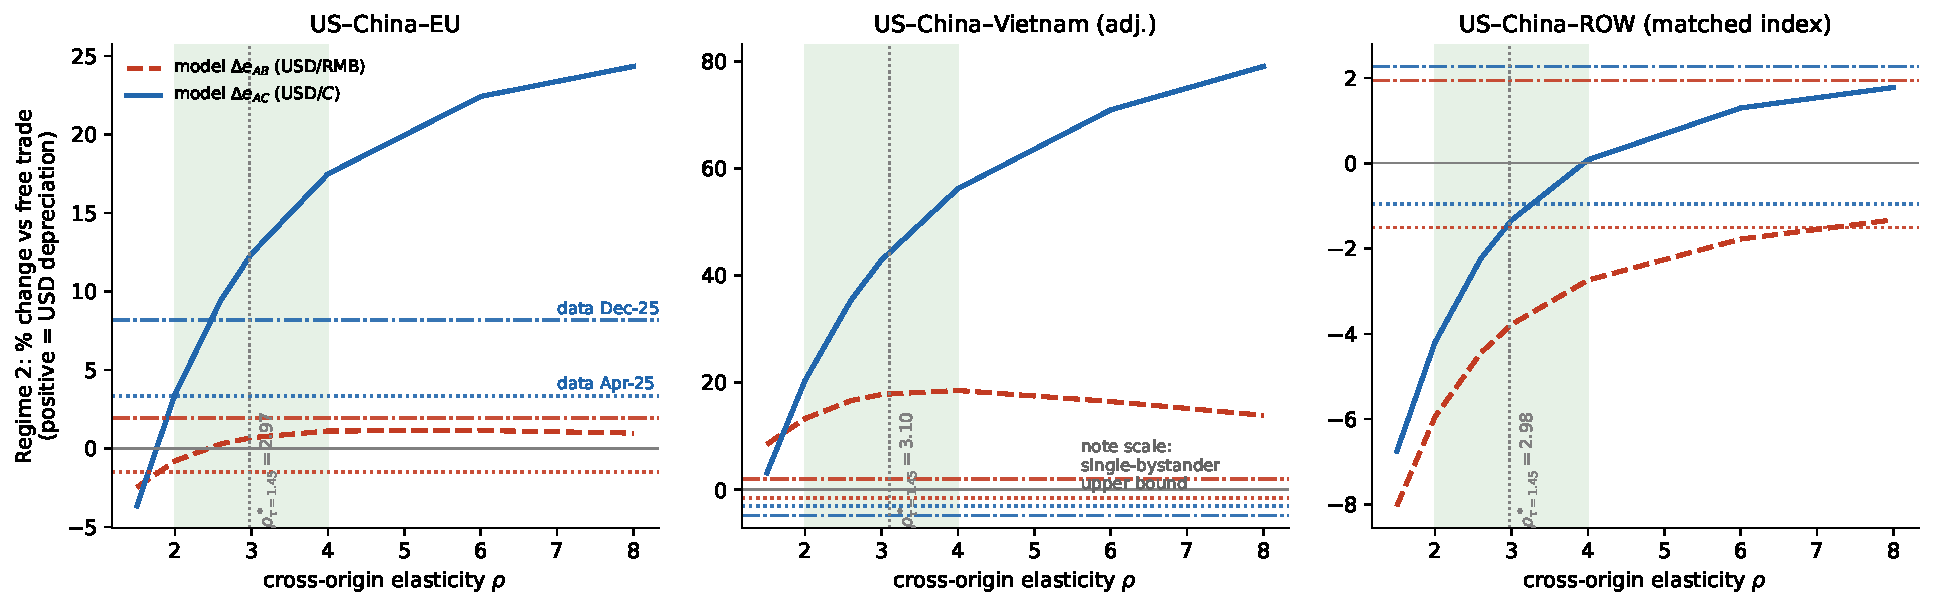
\includegraphics[width=\textwidth]{calibration_nested_results.pdf}
\caption{\rev{Regime-2 model predictions across the cross-origin elasticity grid, against the April 2025 data (each data window is compared to its own tariff regime; the December window appears in the text against Regime 3). Solid: model $\Delta e_{AC}$ (USD against $C$'s currency); dashed: model $\Delta e_{AB}$ (USD/RMB); horizontal dotted lines: observed April 2025 changes relative to the 2024 average, colored to match the corresponding model object. Shaded band: the empirically central cross-origin range $\rho \in [2, 4]$. Vertical dotted line: the configuration's cumulative reversal threshold at $\tau = 1.45$. Positive values denote dollar depreciation. The Vietnam panel is a single-bystander upper bound (see text).}}
\label{fig:results}
\end{figure}

\begin{revblock}
\paragraph{April 2025 against Regime 2.} Consider first the EU configuration, the cleanest available test of the bystander mechanism: the euro floats, the EU faced only the 10 percent baseline in April, and it did not retaliate. At $\rho = 2.0$, the model's Regime-2 prediction is $(\Delta e_{AB}, \Delta e_{AC}) = (-0.80, +3.45)$ percent against April 2025 data of $(-1.51, +3.36)$: both signs and both magnitudes, at a cross-origin elasticity in the center of the empirically supported band. The ROW configuration, evaluated against the matched ex-China index, is consistent at a somewhat higher elasticity: at $\rho = 3.0$ the model predicts $(-3.78, -1.34)$ against April data of $(-1.51, -0.95)$ --- in April the dollar \emph{appreciated} slightly against the ex-China world, and the model reproduces this, because at moderate $\rho$ the asymmetric war plus the 10 percent tariff on $C$ itself leaves the dollar mildly strong against a large bystander.

\paragraph{Vietnam is not a bystander test.} The dollar strengthened against the dong throughout 2025 ($-3.06$ percent in April, $-4.83$ by December), while the trade-war experiment predicts the opposite --- and no defensible elasticity repairs this within the bystander framing (even pricing the announced-but-paused 46 percent April rate on Vietnam, the model has the dong appreciating, because the 145 percent rate on China still dominates). The resolution is that Vietnam was not a bystander: it was itself a principal tariff target --- 46 percent announced on April 2, 20 percent in force from July, equal to the December rate on China. Once Vietnam's actual tariff is used (Regime 3), the model predicts dollar strength against the dong of $3.5$--$4.6$ percent at central elasticities, against $4.8$ percent observed: with near-equal rates on China and Vietnam there is nothing to divert between them, the configuration collapses to the conventional own-tariff case, and the small tariffed country's currency falls. We therefore read the dong as a test of the \emph{classification} --- the model tracks who is tariffed how much --- rather than of the bystander mechanism, for which the euro and the ex-China aggregate are the valid tests. The Vietnam trio otherwise remains a mechanism illustration: with a single bystander one-eighteenth the size of the US, the model routes the entire diversion through one small economy, an upper bound by construction.

\paragraph{December 2025 against Regime 3.} The December window is compared to the rates then in force, and this comparison is deliberately hard for the model: by December the tariff structure was nearly \emph{uniform} (20 percent on China, 15--20 percent on third countries), so the discrimination that powers the diversion mechanism had largely disappeared, and the model's prediction reverts toward the conventional uniform-tariff case --- mild dollar \emph{appreciation} against everyone. At $\rho = 2.6$: EU configuration $(-4.6, -4.9)$, ROW $(-5.6, -6.4)$, Vietnam $(-4.6, -4.6)$. The data: the dong matches ($-4.8$), but the euro ($+8.2$) and the ex-China index ($+2.3$) show substantial dollar \emph{weakness}. The model is explicit about what this means: at December's near-uniform rates, the prevailing tariff structure cannot account for the observed multilateral dollar depreciation through the trade channel. Whatever drove the late-2025 dollar --- expectations that discriminatory escalation would resume, an erosion of the dollar's safe-haven premium \citep{kalemli2025, cardani2025exchange}, monetary policy --- it was not the tariffs then in force. This is the paper's inference discipline cutting in both directions: the same framework that attributes the April pattern to trade fundamentals \emph{declines} to attribute the December pattern to them.

Three quantitative regularities deserve note. First, the model's real-rate predictions track the nominal ones with a modest wedge ($\Delta q_{AC} = +7.6$ against $\Delta e_{AC} = +9.4$ percent in the EU configuration at $\rho = 2.6$), consistent with Section~\ref{sec:impossibility}'s result that the real-rate reversal threshold exceeds the nominal one. Second, each configuration's \emph{cumulative} reversal threshold at the peak bilateral tariff is nearly the same --- $2.97$ (EU), $3.10$ (Vietnam adj.), $2.98$ (ROW) --- so at 2025-scale tariffs the reversal requires only a cross-origin elasticity near $3$, comfortably inside the measured range, in every configuration. Third, under Regime~1 (the isolated tariff) the model concentrates appreciation on the renminbi with an order-of-magnitude smaller move against $C$ ($\Delta e_{AB} = -5.6$, $\Delta e_{AC} = -1.6$ percent in the EU configuration at $\rho = 2.6$, against March data of $-0.91$ and $-0.23$), overpredicting the one-month bilateral magnitude as a long-run model should at a one-month horizon.

Two caveats keep this exercise in proportion. First, monthly exchange-rate observations confront a static balanced-trade model whose predictions are long-run tendencies; exchange-rate disconnect at short horizons \citep{itskhoki2021} cautions against reading any single window as a point test, and the December window in particular shows how much of the exchange rate the trade channel does \emph{not} explain once the tariff structure turns uniform. Second, the three-country design itself bounds what any configuration can capture: a single untariffed aggregate cannot represent simultaneous dollar appreciation against some bystanders and depreciation against others, which is what the cross-section of bilateral rates shows; the configuration-by-configuration results should be read as the model's answer for \emph{that} bystander in isolation. We therefore present the exercise as a disciplined illustration of the mechanism's quantitative shape --- with magnitudes on the scale of the data at empirically central elasticities --- rather than as a validated forecast.
\end{revblock}

\section{Conclusion}
\label{sec:conclusion}

\begin{revblock}
This paper connects two literatures that have not spoken to each other, and draws out what the connection implies for a live policy debate. In the model class behind the conventional tariff--appreciation prediction, the exchange rate is the common-currency relative wage and therefore the bilateral terms of trade --- the object the preferential-trade-agreement literature has studied since Viner --- and a selective tariff is formally a preference in favor of the untariffed partner. The connection went unstated, we argue, for a definite reason: it is invisible in the standard specification. Under a single elasticity of substitution across all tradable varieties, the conventional prediction \emph{survives} multilateralization as a theorem --- a discriminatory tariff cannot depreciate the tariff-imposing country's currency against the untariffed third country at any elasticity under realistic home bias, because a common elasticity strengthens trade diversion and home-versus-import expenditure switching in the same proportion. The reversal exists only once the two margins are separated: the currency depreciates against untariffed partners if and only if the cross-origin elasticity exceeds the closed-form threshold $\rho^* = 3[1 + \alpha_D(\eta-1) - \alpha_T(1-\alpha_D)]$ --- approximately $4$ at US-realistic parameters for marginal tariffs and approximately $3$ at 2025-scale tariffs, inside the range of measured cross-origin elasticities. In a near-symmetric bilateral trade war the ambiguity resolves: both belligerents depreciate against the untariffed bystander, with magnitude increasing in $\rho$. A calibration to the 2025 episode, disciplined by the tariffs in force at each date, matches the April pattern --- modest dollar appreciation against the renminbi alongside a $3$--$4$ percent depreciation against the euro --- at a cross-origin elasticity of about $2$, and explains the dollar's strength against the dong once Vietnam's own tariff is used: the model tracks who is tariffed how much.

These results have direct implications for interpreting exchange-rate movements during tariff episodes, and the implications cut in both directions. Exchange-rate appreciation against a bilateral trading partner is not evidence of broad currency strength, and observed multilateral depreciation during a discriminatory tariff episode cannot be attributed to financial or convenience-yield channels on the strength of the two-country prior alone: real trade channels generate exactly this pattern once cross-origin substitution exceeds the threshold, and generate it unambiguously in a retaliated trade war --- the configuration dependence documented in high-frequency data by \cite{corsetti2025}. But the same framework refuses the attribution when the tariff structure does not support it: by late 2025, with near-uniform rates across China and third countries, the trade channel predicts mild dollar strength, so the year-end dollar weakness must be attributed elsewhere --- to expectations of renewed escalation, safe-haven erosion, or monetary policy. A sign condition that can decline to explain things is, we think, precisely what the attribution debate has been missing.
\end{revblock}

Several directions for future work suggest themselves. A natural extension would embed the mechanisms identified here in a quantitative multi-country trade model with richer bilateral trade flow patterns, input-output linkages, and heterogeneous elasticities across sectors and country pairs. A further extension would introduce nominal rigidities and a financial account, allowing the real exchange rate channels to interact with the monetary and portfolio balance dynamics that dominate exchange rate movements at shorter horizons. Incorporating these features into a unified framework would bring the conceptual results established here closer to a quantitative tool suitable for policy analysis.

\newpage

\addcontentsline{toc}{section}{\bf \small{References}} 
% \bibliographystyle{apa}
\bibliography{references}

\newpage
\begin{appendix}

\section{Two-Country Conventional Wisdom Robustness}
\label{app:robustness}

\paragraph{Alternative demand-side specifications.}
We first examine the robustness of Lemmas~\ref{lem:tariff_monotonicity} and~\ref{lem:er_monotonicity} under a broad class of standard demand systems. The key observation is that tariffs and exchange rates affect demand only through relative prices. As long as import demand is decreasing in its consumer price and export revenues are weakly increasing in export competitiveness, the monotonicity conditions required for the sign of $de/d\tau$ are satisfied. Consider CES (Armington) preferences over tradable goods with elasticity of substitution $\sigma > 0$, with utility separable between tradables and non-tradables. Under the producer-price normalization, the consumer price of imports in country $A$ is $p_M(e,\tau) = (1+\tau)e$. For any $\sigma > 0$, Marshallian import demand is strictly decreasing in $p_M(e,\tau)$, so at a fixed exchange rate an increase in $\tau$ reduces import expenditures while export revenues are locally unaffected, verifying the conditions of Lemma~\ref{lem:tariff_monotonicity}. Holding $\tau$ fixed, a depreciation raises the domestic-currency price of imports and lowers the foreign-currency price of exports, implying falling import expenditures and weakly rising export revenues, which verifies Lemma~\ref{lem:er_monotonicity}. The same logic applies to nested CES preferences that allow for separate elasticities between tradables and non-tradables and across tradable varieties. While tariff-induced income effects may reallocate expenditure between tradables and non-tradables, the monotonic relationship between import demand and its consumer price is preserved as long as the elasticity of substitution across tradables is positive, and exchange-rate movements continue to generate standard expenditure-switching effects. Finally, under quasi-linear preferences, income effects from tariff revenue are eliminated entirely. Import demand depends only on relative prices and remains decreasing in the consumer import price, while export revenues respond monotonically to changes in export competitiveness. The conditions of Lemmas~\ref{lem:tariff_monotonicity} and~\ref{lem:er_monotonicity} therefore hold by construction.

\paragraph{Alternative production-side specifications.}
We next examine alternative production structures that allow wages and output to adjust endogenously. The common feature of these specifications is that tariffs and exchange rates affect production only through their effects on demand and relative prices. Consider production technologies with diminishing returns to labor or sector-specific factors. Under perfect competition, wages adjust to clear labor markets and output responds endogenously to demand shifts. Holding the exchange rate fixed, a higher tariff continues to raise the consumer price of imports in country $A$ and reduce import expenditures. Although wages and output adjust in general equilibrium, these adjustments do not overturn the import-compression effect of the tariff. In particular, since the tariff does not introduce any export-side wedge or subsidy, export revenues are not adversely affected at fixed $e$, so the conditions of Lemma~\ref{lem:tariff_monotonicity} remain satisfied. Holding the tariff fixed, a depreciation raises the domestic-currency price of imports and lowers the foreign-currency price of exports. Under standard regularity conditions, import expenditures fall and export revenues weakly increase, even when wages and output adjust endogenously. Sectoral wage adjustments induced by demand shifts reinforce, rather than offset, the expenditure-switching effects as long as higher export demand raises export-sector wages or output without generating a sufficiently strong increase in marginal costs that would reverse the competitiveness gain. We rule out such counterfactual cases by assuming that export supply is weakly increasing in export prices, under which the requirements of Lemma~\ref{lem:er_monotonicity} are satisfied. A similar argument applies when export supply is endogenous due to capacity constraints or increasing marginal costs: provided that export supply is weakly increasing in the export price faced by foreign consumers, a depreciation raises the value of exports measured in country $A$'s currency while higher import prices reduce import expenditures, so $\mathrm{TB}_{A,e}(e,\tau) > 0$ continues to hold locally.

\paragraph{Alternative fiscal closures and other specifications.}
Finally, we briefly examine additional modeling choices commonly considered in the literature. These specifications differ in how income effects, pricing, or market structure are treated, but they leave unchanged the relative-price channels through which tariffs and exchange rates affect trade flows in the medium to long run. First, consider alternative treatments of tariff revenue. Whether tariff revenue is rebated lump-sum, wasted, transferred abroad, or used to finance government spending, a tariff continues to raise the consumer price of imports at a fixed exchange rate. As long as import demand is decreasing in its consumer price, import expenditures fall at the prevailing exchange rate while export revenues are not adversely affected locally, and a depreciation continues to raise import prices and lower export prices. Hence the conditions of Lemmas~\ref{lem:tariff_monotonicity} and~\ref{lem:er_monotonicity} hold under standard fiscal closures. Second, consider alternative market structures and pricing assumptions, such as monopolistic competition in tradables or local- and dominant-currency pricing. These assumptions primarily affect the degree and timing of exchange rate passthrough. In the short run, incomplete passthrough under dominant-currency pricing may attenuate expenditure-switching effects and delay the adjustment of trade flows. However, once prices adjust, relative prices faced by consumers reflect both the tariff wedge and the exchange rate, and in this flexible-price equilibrium the monotonicity conditions remain valid. Finally, these conclusions are unchanged in simpler or asymmetric environments, including pure-tradables economies or the small open economy limit. In each case, tariffs compress import demand at a fixed exchange rate and exchange-rate movements generate standard expenditure-switching effects. While the magnitude of the exchange rate response may vary across specifications, its sign does not. Taken together, the results in this section show that the appreciation of the tariff-imposing country's currency in a two-country setting is not an artifact of particular assumptions about fiscal policy, market structure, or pricing conventions. Rather, it follows from general monotonicity properties of import and export behavior that hold across a wide range of standard models, once relative prices are allowed to adjust.

\begin{revblock}
\section{The Reversal Threshold at a General Baseline}
\label{app:threshold}

This appendix derives the local response $d\log e_{AC}/d\tau|_{\tau=0}$ at an arbitrary free-trade baseline of the nested model, by linearization in baseline expenditure shares (``hat algebra''). The baseline is described entirely by observables: common-currency incomes $y_i = e_{Ai} w_i L_i$, home shares $h_i$ of each country's tradable expenditure, import-bundle origin shares $b_{ij}$ (the share of origin $j$ in $i$'s import bundle, $\sum_{j \neq i} b_{ij} = 1$), and the tradable expenditure share $\alpha_T$.

Let $\nu_j = \log e_{Aj}$ (with $\nu_A = 0$) and let $s_{ij}$ denote the share of country $i$'s total income spent on variety $j$, so $s_{ii} = \alpha_T h_i$ and $s_{ij} = \alpha_T (1-h_i) b_{ij}$ for $j \neq i$. Log-differentiating the nested CES demand system at the baseline, with $d\log p_{ij} = d\nu_j + \mathbf{1}\{(i,j)=(A,B)\}\, d\tau$:
\begin{align*}
d\log P_{M_i} &= \sum_{j \neq i} b_{ij}\, d\log p_{ij}, \qquad
d\log P_{T_i} = h_i\, d\log p_{ii} + (1-h_i)\, d\log P_{M_i}, \\
d\log s_{ii} &= (1-\eta)\left( d\log p_{ii} - d\log P_{T_i} \right), \\
d\log s_{ij} &= (1-\rho)\left( d\log p_{ij} - d\log P_{M_i} \right) + (1-\eta)\left( d\log P_{M_i} - d\log P_{T_i} \right), \quad j \neq i,
\end{align*}
and $d\log I_i = d\nu_i + \mathbf{1}\{i = A\}\, s_{AB}\, d\tau$, where the second term is the first-order tariff-rebate effect. Totally differentiating the two independent balanced-trade conditions
\[
\mathrm{TB}_i = \sum_{k \neq i} \frac{s_{ki}\, I_k}{1+\tau_{ki}} - \sum_{j \neq i} \frac{s_{ij}\, I_i}{1+\tau_{ij}}, \qquad i \in \{B, C\},
\]
at $\tau = 0$ (the term $-s_{AB}\, y_A\, d\tau$ from $d[1/(1+\tau_{AB})]$ enters $B$'s export revenue) yields a linear $2\times 2$ system in $(d\nu_B, d\nu_C)$. Solving by Cramer's rule:

\begin{proposition}[General-baseline threshold]
\label{prop:general_threshold}
At any free-trade baseline,
\[
\left.\frac{d\log e_{AC}}{d\tau}\right|_{\tau=0} = \frac{N(\rho)}{D},
\qquad
N(\rho) = c_2\,\rho^2 + c_1\,\rho + c_0,
\]
where $D > 0$ at a locally stable equilibrium and the coefficients $c_2, c_1, c_0$ depend only on $(y_i, h_i, b_{ij}, \alpha_T, \eta)$. The leading coefficient is
\[
c_2 = b_{AB}\, b_{AC}\, b_{CA}\, b_{CB}\, (1-h_A)(1-h_C)\, y_A\, y_C \;>\; 0,
\]
so $N$ is an upward parabola and the reversal threshold is its larger root $\rho^*$: country $A$ depreciates against the untariffed third country if and only if $\rho > \rho^*$, at any baseline. All three coefficients share the factor $b_{AB}(1-h_A)\,y_A$ --- country $A$'s import exposure to $B$, without which the experiment is vacuous --- and $c_0$ contains the factor $1 + h_A(\eta-1) - \alpha_T(1-h_A)$, the symmetric threshold $\rho^*/3$ with $h_A$ in place of $\alpha_D$.
\end{proposition}

At the symmetric point ($h_i = \alpha_D$, $b_{ij} = 1/2$, $y_i = 1$) the expression reduces exactly to Proposition~\ref{prop:threshold}. The full coefficient expressions are unwieldy in print and are provided, together with a symbolic derivation and a numerical validation against nonlinear equilibrium solves (agreement to five decimal places at the size configurations of Table~\ref{tab:rhostar_grid}), in the replication package.
\end{revblock}

\section{Calibration Details}
\label{app:calibration}

\subsection*{Tariff Rate Calibration}
\label{app:tariffs}
All tariff rates are measured as incremental ad valorem rates above the pre-2025 baseline, which we treat as free trade. Rates are sourced from official executive orders, Federal Register notices, and contemporaneous policy documentation.

\paragraph{Regime 1 (Fentanyl-related tariffs).} The 20 percent tariff on Chinese imports ($\tau_{AB} = 0.20$) reflects the cumulative incremental tariffs imposed on China in February and March 2025 under the International Emergency Economic Powers Act (IEEPA) on fentanyl-related grounds, prior to the Liberation Day announcement. China did not impose retaliatory tariffs during this period, giving $\tau_{BA} = 0$. No incremental tariff was imposed on third countries at this stage, so $\tau_{AC} = \tau_{CA} = 0$ across all configurations.

\paragraph{Regime 2 (Peak escalation).} Following the Liberation Day announcement of April 2, 2025, the US imposed country-specific reciprocal tariffs on most trading partners effective April 9. However, on April 9 the administration suspended all country-specific reciprocal tariffs for 90 days for every country except China, leaving only a universal 10 percent baseline tariff in place for non-China partners. The effective incremental US tariff on China at the peak of escalation was 145 percent ($\tau_{AB} = 1.45$), combining the Liberation Day reciprocal rate of 34 percent with the pre-existing fentanyl tariffs and subsequent escalation steps. China retaliated with a cumulative tariff of 125 percent on US goods ($\tau_{BA} = 1.25$). For all third-country configurations, the US tariff on $C$ is set to the 10 percent baseline that remained in effect after the April 9 pause ($\tau_{AC} = 0.10$). Neither the EU nor Vietnam imposed retaliatory tariffs on the US during this period, so $\tau_{CA} = 0$.

\rev{\paragraph{Regime 3 (Late 2025).} The May 12 Geneva agreement suspended the peak bilateral rates: the US rate on China fell to 30 percent incremental (10 percent reciprocal plus 20 percent fentanyl-related), and China's retaliation to 10 percent. On November 10, 2025, following the October--November agreement, the fentanyl-related rate was halved, leaving the US rate on China at 20 percent ($\tau_{AB} = 0.20$) and China's at 10 percent ($\tau_{BA} = 0.10$) through the December window. Third-country rates reflect the 2025 framework agreements: 15 percent on EU goods (July framework), 20 percent on Vietnamese goods (July agreement), and approximately 15 percent for the ROW aggregate (a rough trade-weighted average of the 10 percent baseline, the 15 percent floor for surplus countries, and higher country-specific rates). No retaliation by the EU or Vietnam ($\tau_{CA} = 0$).}

\subsection*{Expenditure Shares}
Expenditure shares are calibrated from 2024 world goods export shares (WTO), with the nontradable share fixed at $\alpha_N = 0.60$ to match the broad cross-country average. Letting $s_j$ denote country $j$'s share of world goods exports, tradable shares are constructed as
\[
\alpha_{T_j} = 0.40 \times \frac{s_j}{s_A + s_B + s_C},
\]
normalizing within each configuration so that shares sum to one. The underlying export shares are $s_A = 8.4\%$ (US), $s_B = 14.3\%$ (China), $s_C = 12.0\%$ (EU), $1.6\%$ (Vietnam), and $77.2\%$ (ROW), where the ROW share is computed as world exports minus the US and China. Because the normalization denominator depends on $s_C$, the values of $\alpha_{T_A}$ and $\alpha_{T_B}$ differ across configurations; the resulting calibration targets are reported in Table~\ref{tab:calibration}. Preference parameters are assumed common across countries, so the same shares apply to $A$, $B$, and $C$.

\subsection*{Labor Endowments}
Labor endowments are set proportional to 2024 GDP at purchasing power parity (PPP), normalizing $L_A = 1$ for the US. PPP-based weights are appropriate because the model abstracts from price level differences across countries, and PPP GDP provides a better measure of relative economic size in volume terms than nominal GDP at market exchange rates. The source figures from the IMF World Economic Outlook \citep{imf2024weo} are: United States \$29.2 trillion, China \$35.3 trillion, European Union \$25.1 trillion, and Vietnam \$1.6 trillion (all in 2024 international dollars), giving $L_B = 1.21$, $L_C^{\mathrm{EU}} = 0.86$, and $L_C^{\mathrm{VNM}} = 0.055$. For the ROW configuration, $L_C^{\mathrm{ROW}}$ is computed as world PPP GDP minus the US and China, giving \$167.0 - \$29.2 - \$35.3 = \$102.5 trillion and $L_C^{\mathrm{ROW}} = 3.51$.

\subsection*{Elasticity of Substitution}
The elasticity of substitution within the tradable bundle is set to $\sigma = 6$ for the EU configuration, $\sigma = 8$ for Vietnam, and $\sigma = 2$ for the ROW configuration. For the EU, the value $\sigma = 6$ is anchored on the cross-origin central estimate from \citet{amiti2019impact}, which yields a preferred elasticity near six across a broad range of manufactured goods imported by the US. The EU value reflects the China Shock 2.0 narrative, under which Chinese manufacturing increasingly competes with European industrial and machinery exports in US import markets. For Vietnam, $\sigma = 8$ reflects Vietnam's deep integration into Chinese supply chains as an assembly and re-export platform \citep{fajgelbaum2024trade}, making Vietnamese and Chinese exports to the US close substitutes at the product level and warranting an elasticity above the cross-origin average. For the ROW aggregate, $\sigma = 2$ reflects the attenuation of bilateral substitution patterns by aggregation across a large and heterogeneous set of trading partners \citep{fajgelbaum2020return, feenstra2018}.

\section{Extended Calibration Results}
\label{app:extended_calibrations}

This appendix presents calibration parameters and model-vs-data comparisons for eight third-country configurations: the European Union and Vietnam \rev{(under the same parameter values as the main text)}, plus Japan, South Korea, Mexico, Canada, Taiwan, and India. For each configuration, $\sigma$ is assigned based on the nature of the bilateral trading relationship with China in US import markets. EU and Vietnam are included for completeness alongside the additional configurations. All data are sourced as described in Appendix~\ref{app:calibration}; observed exchange rate changes are percent changes relative to the 2024 annual average.

\rev{The broad pattern of fit mirrors what is discussed for the three main configurations in Section~\ref{sec:calibration}. Under Regime~1 the model predicts dollar appreciation against both the RMB and every third-country currency, concentrated on the RMB; the data match the direction against the RMB and most third currencies, with the model overpredicting bilateral USD/RMB magnitudes at the one-month horizon. Under Regime~2 the model predicts modest dollar appreciation against the RMB (matching the observed $-1.51$ percent in sign) in all configurations except Canada, alongside USD depreciation against every third-country currency, consistent with the trade-war mechanism. The data confirm the third-currency depreciation for the euro and the yen; for most other trading partners the financial risk-off channel --- which the model abstracts from by design --- dominates at the April 2025 horizon, and the model's predicted depreciation magnitudes for small open economies (Canada, Taiwan, India) remain far too large, reflecting the counterfactual home-bias implications of world-export-share preference weights discussed in Section~\ref{sec:calibration}. South Korea and Taiwan follow the same pattern as the other non-safe-haven currencies; their divergence reflects their deep integration in US-oriented trade and supply chains rather than any emerging-market classification.}

\begin{table}[htbp]
\centering
\caption{Calibration parameters by third-country configuration. $\alpha_N = 0.60$ throughout. Tradable shares are constructed from 2024 WTO world goods export shares; labor endowments from IMF WEO 2024 PPP GDP ($L_A = 1$). $\sigma$ assigned as described in main text and notes below.}
\label{tab:app_params}
\vspace{4pt}
\begin{tabular}{lcccccc}
\hline\hline
Country $C$ & $\sigma$ & $\alpha_{T,A}$ & $\alpha_{T,B}$ & $\alpha_{T,C}$ & $\alpha_N$ & $L_C / L_A$ \\
\hline
European Union  & 6 & 0.097 & 0.165 & 0.138 & 0.600 & 0.860 \\
Japan           & 4 & 0.129 & 0.220 & 0.051 & 0.600 & 0.226 \\
South Korea     & 5 & 0.132 & 0.225 & 0.043 & 0.600 & 0.103 \\
Mexico          & 5 & 0.132 & 0.224 & 0.044 & 0.600 & 0.113 \\
Canada          & 2 & 0.134 & 0.228 & 0.038 & 0.600 & 0.086 \\
Vietnam         & 8 & 0.138 & 0.235 & 0.026 & 0.600 & 0.055 \\
Taiwan          & 3 & 0.135 & 0.230 & 0.035 & 0.600 & 0.058 \\
India           & 3 & 0.137 & 0.233 & 0.031 & 0.600 & 0.497 \\
\hline\hline
\end{tabular}
\begin{tablenotes}
\footnotesize
\item \textit{Notes:} $\sigma$ values: EU ($\sigma=6$) anchored on Amiti, Redding \& Weinstein (2019) cross-origin central estimate; Japan ($\sigma=4$) advanced autos and machinery with limited Chinese overlap; South Korea ($\sigma=5$) and Mexico ($\sigma=5$) meaningful product-level overlap in electronics and manufacturing; Canada ($\sigma=2$) commodity-heavy exports (energy, mining) with low substitutability; Vietnam ($\sigma=8$) deep supply-chain integration with China; Taiwan ($\sigma=3$) semiconductor-dominant with limited aggregate substitutability; India ($\sigma=3$) growing manufacturing base with limited current overlap.
\end{tablenotes}
\end{table}

\begin{table}[htbp]
\centering
\caption{Model-implied and realized exchange rate changes by regime. Model columns report percent changes relative to the free-trade benchmark; data columns report percent changes relative to the 2024 annual average. $\Delta e_{AB}$: USD/RMB; $\Delta e_{AC}$: USD/$C$-currency; $\Delta e_{BC}$: RMB/$C$-currency. Positive values denote depreciation of the first currency. \rev{Model values are computed under the corrected demand system of Section~\ref{sec:threecountry} (realized-share tariff revenue and share-linear weights).}}
\label{tab:app_regimes}
\vspace{4pt}
\begin{tabular}{l
    r r r
    @{\hspace{0.6cm}}
    r r r}
\hline\hline
 & \multicolumn{3}{c}{Model (\%)} & \multicolumn{3}{c}{Data (\%)} \\
Country $C$ & $\Delta e_{AB}$ & $\Delta e_{AC}$ & $\Delta e_{BC}$ & $\Delta e_{AB}$ & $\Delta e_{AC}$ & $\Delta e_{BC}$ \\
\hline
\multicolumn{7}{l}{\textit{Panel A: Regime 1 (Fentanyl-related tariffs, March 2025)}} \\[2pt]
European Union  & \rev{$-5.39$} & \rev{$-0.44$} & \rev{$+5.23$} & $-0.91$ & $-0.23$ & $+0.69$ \\
Japan           & \rev{$-7.95$} & \rev{$-1.14$} & \rev{$+7.40$} & $-0.91$ & $+1.42$ & $+2.35$ \\
South Korea     & \rev{$-8.27$} & \rev{$-0.92$} & \rev{$+8.02$} & $-0.91$ & $-6.46$ & $-5.60$ \\
Mexico          & \rev{$-8.22$} & \rev{$-0.91$} & \rev{$+7.96$} & $-0.91$ & $-10.00$ & $-9.17$ \\
Canada          & \rev{$-9.60$} & \rev{$-2.80$} & \rev{$+7.52$} & $-0.91$ & $-4.61$ & $-3.73$ \\
Vietnam         & \rev{$-8.27$} & \rev{$-0.49$} & \rev{$+8.48$} & $-0.91$ & $-1.93$ & $-1.03$ \\
Taiwan          & \rev{$-9.04$} & \rev{$-1.79$} & \rev{$+7.98$} & $-0.91$ & $-2.73$ & $-1.84$ \\
India           & \rev{$-7.91$} & \rev{$-1.55$} & \rev{$+6.91$} & $-0.91$ & $-3.43$ & $-2.54$ \\[4pt]
\multicolumn{7}{l}{\textit{Panel B: Regime 2 (Peak escalation, April 2025)}} \\[2pt]
European Union  & \rev{$-2.50$} & \rev{$+3.57$}  & \rev{$+6.23$}  & $-1.51$ & $+3.36$  & $+4.94$ \\
Japan           & \rev{$-1.57$} & \rev{$+9.97$}  & \rev{$+11.72$} & $-1.51$ & $+4.55$  & $+6.15$ \\
South Korea     & \rev{$-2.26$} & \rev{$+7.59$}  & \rev{$+10.08$} & $-1.51$ & $-5.66$  & $-4.21$ \\
Mexico          & \rev{$-2.27$} & \rev{$+7.55$}  & \rev{$+10.04$} & $-1.51$ & $-9.33$  & $-7.94$ \\
Canada          & \rev{$+1.12$} & \rev{$+16.87$} & \rev{$+15.58$} & $-1.51$ & $-2.29$  & $-0.79$ \\
Vietnam         & \rev{$-3.39$} & \rev{$+2.42$}  & \rev{$+6.02$}  & $-1.51$ & $-3.06$  & $-1.57$ \\
Taiwan          & \rev{$-0.27$} & \rev{$+14.62$} & \rev{$+14.92$} & $-1.51$ & $-2.00$  & $-0.50$ \\
India           & \rev{$-0.58$} & \rev{$+12.67$} & \rev{$+13.33$} & $-1.51$ & $-2.31$  & $-0.81$ \\
\hline\hline
\end{tabular}
\end{table}

\end{appendix}


\end{document}